\documentclass[12pt,letterpaper,final, openany]{scrbook}
\usepackage[utf8]{inputenc}
\usepackage[spanish]{babel}
\usepackage{amsmath}
\usepackage{amsfonts}
\usepackage{amssymb}
\usepackage{graphicx}
\graphicspath{{figures/}}
\usepackage{tocloft}
\usepackage[table]{xcolor}
\usepackage[left=3cm,right=3cm,top=3cm,bottom=2cm]{geometry}
\usepackage{float}
\usepackage{caption}
\usepackage{subcaption}
\usepackage{xcolor}
\usepackage{hyperref}
\hypersetup{bookmarksopen,bookmarksnumbered,colorlinks=true,linkcolor=black,citecolor=blue,urlcolor=blue}
\usepackage{setspace}
\usepackage{xurl}

%\usepackage[backend=biber,style=ieee,]{biblatex}
%\addbibresource{referencias2.bib} %Import the bibliography file
\setlength{\parindent}{0pt}

\makeatletter
\author{Maximiliano Garavito Chtefan}\let\Author\@author
\title{Modelo semi-supervisado de redes neuronales convolucionales equivariantes para la segmentación y clasificación de imágenes histopatológicas}\let\Title\@title
\makeatother

\addto\captionsspanish{\renewcommand{\contentsname}{Contenido}}
\renewcommand{\cftsecleader}{\cftdotfill{\cftdotsep}}
\usepackage[hang]{footmisc}
\setlength\footnotemargin{8pt}



\begin{document}
\pagestyle{plain}


%% PORTADA %%%%%%%%%%%%%%%%%%%%%%%%%%%%%%%%%%%%%%%%%%%%%%%%%%%%%%%%%%%%%%%%%%
\begin{center}
\vspace*{0.2cm}
%{\fontsize{18}{22}\selectfont \textbf{\Title}}\\[1.5cm]
%{\setstretch{5}\fontsize{18pt}{50pt}\selectfont\textbf\Title}\\[1.5cm]
\Large\textbf{\Title }\\[2cm]
\large\textbf{Propuesta de Investigación - Plan de trabajo}\\[2cm]
\Large\Author\\[2cm]
\large\textbf{Director:}\\
\large{David Romo Bucheli, Ph.D}\\[0.5cm]
\normalsize Universidad Industrial de Santander\\
Facultad de Ingenierías Fisicomecánicas\\
Escuela de Ingeniería de Sistemas e Informática\\
Bucaramanga\\
2024\\[1.5cm]
\begin{center}

\includegraphics[width=0.8\textwidth]{logos.jpg}
\end{center}
%\vspace*{1.5cm}
\pagenumbering{gobble}
\end{center}


%% CONTENIDO %%%%%%%%%%%%%%%%%%%%%%%%%%%%%%%%%%%%%%%%%%%%%%%%%%%%%%%%%%%%%%%%
\setcounter{tocdepth}{2}
\tableofcontents
%% RESUMEN %%%%%%%%%%%%%%%%%%%%%%%%%%%%%%%%%%%%%%%%%%%%%%%%%%%%%%%%%%%%%%%%%%
\newpage
\pagenumbering{arabic}
\setcounter{page}{1}
\addcontentsline{toc}{section}{Resumen}
\begin{center}
\Large\textbf{RESUMEN}\\[20pt]
\end{center}
\textbf{Título:} \Title.\footnotemark[1]

\textbf{Autor:} \Author.\footnotemark[2]

\textbf{Palabras Clave:} Redes neuronales convolucionales equivariantes, imágenes histopatológicas, procesamiento de imágenes, aprendizaje semi-supervisado

\textbf{Objetivo General:} Desarrollar un modelo semi-supervisado de redes neuronales convolucionales equivariantes para la segmentación y clasificación de imágenes histopatológicas.

\textbf{DESCRIPCIÓN:}

%La patología digital representa un cambio de paradgima en el enfoque tradicional de diagnóstico médico (Baxi et al., 2022). Dentro de la medicina contemporánea ``los avances tecnológicos en curso remodelan constantemente las prácticas de atención médica" (Kiran et al., 2023, p. 1). Por lo que, el desarrollo de la patología digital no es una moda, sino un logro transformador (Kiran, et al., 2023) que permite introducir "una combinación de tecnología de punta, análisis de datos y experiencia clínica que puede transformar significativamente la forma en que se brinda la atención al paciente" (Kiran et al., 2023, p. 1).

La patología digital representa un cambio de paradigma en el enfoque tradicional de diagnóstico médico. Dentro de la medicina contemporánea los avances tecnológicos en curso remodelan constantemente las prácticas de atención médica. Por lo que, el desarrollo de la patología digital es un logro transformador que permite introducir una combinación de dispositivos electrónicos de punta, como los escáneres de  láminas histológicas, análisis de datos y experiencia clínica que puede transformar significativamente la forma en que se brinda la atención al paciente.

%Dentro de las aplicaciones de la patología digital, una de las que mayor acogida e interés ha provocado han sido las que respectan al cáncer, dado que es una de las principales causas de muerte a nivel global, ya que, "se estima que hubo 20 millones de nuevos casos de cáncer y 10 millones de muertes por cáncer. La carga del cáncer aumentará aproximadamente en un 60\% durante las próximas dos décadas, lo que afectará aún más a los sistemas de salud, a las personas y a las comunidades" (Organización Panamericana de la Salud, 2023, párr. 5)
Dentro de las aplicaciones de la patología digital, una de las que mayor acogida e interés ha provocado han sido las que respectan al cáncer. Esto es debido a que es una de las principales causas de muerte a nivel global. La carga del cáncer aumentará aproximadamente en un 60\% durante las próximas dos décadas, lo que afectará aún más a los sistemas de salud, a las personas y a las comunidades.

Dado esto, se requiere un nuevo enfoque como el uso de modelos de inteligencia artificial (IA), que optimizan y aceleran los métodos actuales. Aunque, se han desarrollado proyectos de aprendizaje automático dentro del ámbito de la patología digital, la limitada disponibilidad de imágenes anotadas y segmentadas obstaculiza los procesos de aprendizaje profundo, pues realizar estos procesos de anotación exigen gran demanda de tiempo y esfuerzo por parte de los patólogos. Hasta ahora los métodos tradicionales de aprendizaje profundo han solucionado estos problemas con el uso de aumento de datos, que consiste en generación de datos nuevos a partir de los que hay, pero este proyecto pretende mostrar el uso de representaciones equivariantes en los modelos de aprendizaje profundo, que permitirían una representación estable y eficaz de imágenes en patología digital.

Por esto, se propone un modelo de aprendizaje profundo semi-supervisado de redes neuronales equivariantes que permitan optimizar el tiempo y los recursos de pre-procesamiento, pero también disminuir las limitaciones que tienen los patólogos al implementar proyectos de análisis automático.



\footnotetext[1]{Tesis.}
\footnotetext[2]{Facultad de Ingenierías Físico-mecánicas. Escuela de Ingeniería de Sistemas e Informática. Director: David Romo Bucheli, Ph.D}


%% ABSTRACT %%%%%%%%%%%%%%%%%%%%%%%%%%%%%%%%%%%%%%%%%%%%%%%%%%%%%%%%%%%%%%%%%
\newpage
\addcontentsline{toc}{section}{Abstract}
\begin{center}
	\Large\textbf{ABSTRACT}\\[20pt]
\end{center}
\textbf{Title:} Semi-supervised model of equivariant convolutional neural networks for segmentation and classification of histopathological images\footnotemark[1]

\vspace*{5mm}

\textbf{Author:} \Author.\footnotemark[2] \\

\textbf{Keywords:} equivariant convolutional neural networks, Histopathological image, digital image processing, semi-supervised learning \\



\textbf{General Objective:}
 Develop a semi-supervised model of equivariant convolutional neural networks for the segmentation and classification of histopathological images.


\textbf{DESCRIPTION:}

Digital pathology represents a paradigm shift in the traditional approach to medical diagnosis. Within contemporary medicine, ongoing technological advances are constantly reshaping healthcare practices. Therefore, the development of digital pathology is a transformative achievement that allows for the introduction of a combination of cutting-edge electronic devices, such as histology slide scanners, data analytics, and clinical expertise that can significantly transform the way patient care is delivered.
Among the applications of digital pathology, one of the most popular and interesting has been that regarding cancer. This is because it is one of the leading causes of death globally. The burden of cancer will increase by approximately 60\% over the next two decades, further affecting healthcare systems, individuals, and communities.

Given this, a new approach is required, such as the use of artificial intelligence (AI) models, which optimize and accelerate current methods. Although machine learning projects have been developed within the field of digital pathology, the limited availability of annotated and segmented images hinders deep learning processes, since performing these annotation processes requires a great deal of time and effort from pathologists. Until now, traditional deep learning methods have solved these problems by using data augmentation, which consists of generating new data from existing data, but this project aims to show the use of equivariant representations in deep learning models, which would allow a stable and effective representation of images in digital pathology.

For this reason, a semi-supervised deep learning model of equivariant neural networks is proposed that allows optimizing pre-processing time and resources, but also reducing the limitations that pathologists have when implementing automatic analysis projects.

\footnotetext[1]{Research Work.}
\footnotetext[2]{Faculty of Physics-Mechanics Engineering. School of Systems Engineering and Informatics. Advisor: David Romo Bucheli, Ph.D.}


%% INTRODUCCIÓN %%%%%%%%%%%%%%%%%%%%%%%%%%%%%%%%%%%%%%%%%%%%%%%%%%%%%%%%%%%%%
\newpage
\chapter{Introducción}

La patología digital es uno de los avances tecnológicos con mayor impacto para diagnostico de enfermedades \cite{pallua_future_2020}, pues a diferencia de la patología tradicional, esta permite el análisis de imágenes sin la limitación de la interacción directa de patólogo-microscopio, lo que además posibilita la colaboración inter-patólogo para diagnósticos complicados. Es importante resaltar las enormes posibilidades que brinda la implementación de este nuevo paradigma dentro del diagnóstico clínico. Es necesario apuntar que, ``la adopción de la patología digital estuvo motivada por una doble necesidad. La creciente tasa de expansión de los datos médicos que ha requerido el desarrollo de métodos más eficientes y escalables para la gestión de datos. Además, la búsqueda de una mayor precisión y uniformidad en los diagnósticos ha llevado a la investigación de soluciones basadas en la tecnología"\cite{kiran_digital_nodate}. El anterior es el contexto general dentro del cual el presente proyecto ha surgido, mismo enfocado en la aplicación de la patología digital en el diagnostico del cáncer, que es el nombre común que recibe un conjunto de enfermedades relacionadas en las que se observa un proceso descontrolado en la división de las células del cuerpo. Pues una de las aplicaciones de la patología digital en la practica médica y prognosis para el paciente cuyo mayor impacto tiene, es el diagnostico de este tipo de enfermedad. Esto se debe a que es uno de los problemas de salud pública con mayor incidencia en el mundo: En Colombia el cáncer fue la segunda causa de muerte durante el periodo 2007-2013. Con aproximadamente 33.538 defunciones anuales, lo que representó el  17,1\% de la mortalidad del país \cite{pardo_c_atlas_2017} y también la segunda causa de muerte en los Estados Unidos\cite{sung_global_2021}. Por otro lado, la detección del cáncer conlleva costos elevados y demanda rapidez en el diagnóstico para una detección temprana, debido a que esta enfermedad puede progresar de manera agresiva y tener un desenlace mortal para el paciente. Por último, el cáncer presenta la particularidad de que los tejidos presentan alta variabilidad, por lo que requiere de un elevado grado de entrenamiento por parte de patólogos expertos para hacer el diagnóstico. Todo esto hace que el cáncer sea una de las enfermedades que mayores problemas presenta dentro el proceso de diagnóstico.

Asimismo, es importante tener en cuenta que el proceso para realizar un diagnóstico de cáncer consiste en tomar una muestra, llamada biopsia, del tejido que presenta neoplasia, para ser preparada en un porta-objetos para su posterior análisis en microscopio por parte de un patólogo. La dificultad de la revisión a profundidad y sistemática de una muestra, hace que la detección se haga inicialmente viendo estructuras a baja magnificación que posteriormente se amplían y estudian a alta magnificación para hacer el diagnostico apropiado. Sin embargo, aún con el proceso exhaustivo de entrenamiento que reciben los patólogos, existe una significativa variabilidad inter-patólogo en los
resultados. Así, patólogos distintos frecuentemente difieren en el diagnóstico de una misma muestra. Por ejemplo, la concordancia sobre el grado tumoral del carcinoma de ovario ha sido reportado con un coeficiente kappa de 0,25 para 664 tumores \cite{matsuno_agreement_2013}; El grado fue moderadamente reproducible en cuatro ensayos (N = 10, 10, 19, 10) con muestras del Cooperative Breast Cancer Tissue Resource (kappa = 0,50-0,59) \cite{meyer_breast_2005}. Por otro lado, en un estudio de 350 pacientes, se encontró que la graduación  histopatológica del cáncer de próstata presentó un kappa de 0.67 \cite{noauthor_prostate_nodate}, mostrando con esto un elemento subjetivo en el diagnóstico.

Para ayudar a mitigar este problema, en el estado del arte se han propuesto herramientas computacionales que puedan dar soporte al diagnóstico, pero analizar muestra teniendo en cuenta estructuras más pequeñas y más dispersas que podrían pasar desapercibidas para un patólogo (algo de particular interés para los casos de detección temprana de cáncer) presenta retos computacionales particulares, como lo son el manejo de imágenes de 100,000x100,000 píxeles con una baja densidad de píxeles asociados a un cáncer particular \cite{niazi_digital_2019} \cite{wang_managing_2012}. Debido a lo anterior, la motivación de este proyecto es el desarrollo de modelos automáticos de detección para soportar el diagnóstico en imágenes histopatológicas propendiendo por la disminución de la variabilidad inter-sujeto.


%La dificultad para realizar la segmentación de estas muestras radica en que gran parte de las imágenes no contienen información relevante. Pues, en una muestra que contiene cientos de células solo algunas van a presentar proceso de mitosis (que se ve en la intensidad del color del tinte aplicado a la muestra). Además, las geometrías de las células son muy diversas, sin mencionar que el cáncer en sí mismo agrega más variabilidad, pues presenta atipia nuclear (variaciones en la forma del núcleo de la célula).
Es importante notar que, bajo un enfoque de entrenamiento supervisado, se requiere de una cantidad elevada de imágenes debidamente anotadas o segmentadas, siendo este proceso de anotación  altamente complejo y que además requiere de tiempos prolongados haciéndolo inviable económicamente debido a la cantidad de horas de patólogo profesional que requiere. Lo anterior hace que la cantidad de imágenes debidamente anotadas sea muy limitada, por lo que la respuesta “natural” de hacer redes neuronales grandes y profundas resulte casi imposible en la práctica. Precisamente para solucionar este problema se propone un régimen de entrenamiento semi-supervisado, pues existe la posibilidad de aumentar la cantidad de imágenes sin anotación asociadas a una patología concreta durante el entrenamiento. De esta manera, las imágenes no anotadas pueden servir como un paso no supervisado del entrenamiento, antes de la etapa de entrenamiento supervisado con una cantidad limitada de imágenes anotadas por expertos.
\\
Para resolver este problema de extracción eficiente de información con pocos datos anotados, se propone diseñar una red neuronal convolucional equivariante a la acción del Grupo Euclidiano (rotaciones y reflexiones). Esta decisión se debe a que estas redes (equivariantes a la acción de un grupo) maximizan la extracción de información cuando se conocen simetrías que la señal presenta \cite{elesedy_provably_2021}. %La elección del Grupo Euclidiano como herramienta para llevar a cabo esta tarea de extracción de información con pocos datos se debe a que es el grupo compuesto por las transformaciones geométricas constituidas por traslaciones, rotaciones y reflexiones - mismas simetrías que presentan las imágenes histopatologicas, ya que estas no tienen una orientación preferida, es decir, las estructuras a analizar se pueden trasladar, rotar o reflejar sin dejar de ser las mismas estructuras. A diferencia de las redes convolucionales usuales, que son (famosamente) equivariantes solamente a traslaciones, una simetría que presenta la mayoría de imágenes naturales. Tal y como afirma Cesa ``La razón fundamental para el desarrollo de redes equivariantes, y la razón de su éxito, es la explotación de las simetrías en los datos. Sin embargo, muchas tareas interesantes se caracterizan sólo por pocas simetrías, si es que hay alguna, en sus patrones, lo que limita las posibles aplicaciones de tales modelos. Además, la cantidad de simetrías puede cambiar al observar las señales contenidas en los datos a diferentes escalas” (Cesa, 2020). Cabe resaltar que las redes equivariantes, son, en general, convolucionales, pues Cohen \& Weiler (Cohen, et al. 2019) demostraron que la convolución en grupos es una operación suficiente y necesaria para todas las funciones lineales en este tipo de redes.
\\
En resumen, el presente trabajo pretende implementar y evaluar un modelo de aprendizaje profundo semi-supervisado basado en redes neuronales convolucionales equivariantes para el análisis de imágenes histopatológicas, buscando una representación robusta, aún con una cantidad limitada de datos.
%% FUNDAMENTOS Y TRABAJO PREVIO %%%%%%%%%%%%%%%%%%%%%%%%%%%%%%%%%%%%%%%%%%%%%%
\newpage
\chapter{Fundamentos y Trabajos Previos}

%%\section{Fundamentos}

En la presente sección se hace una breve descripción de los aspectos teóricos que soportan el trabajo de investigación. Esta sección se divide en dos subsecciones: la primera hace una revisión de temas asociados a la patología digital, lo cual incluye, el análisis automático de imágenes histopatológicas; la segunda, hace una revisión sobre lo relacionado con el modelo de redes neuronales equivariantes.

\section{Patología digital}

La patología digital refiere a un conjunto de herramientas y sistemas destinados a la adquisición, gestión y diagnóstico de portaobjetos de patología en un entorno digital (Song et al., 2023)\cite{song_artificial_2023}. Inicialmente la revolución de la patología tradicional comenzó por el desarrollo de la imagen completa del portaobjeto. Esto facilitó realizar diagnósticos asistidos por computadora. Pero, actualmente el entrenamiento de algoritmos de inteligencia artificial promete la posibilidad de explorar y extraer información más allá de la percepción visual humana \cite{baxi_digital_2022}.

La idea básica consiste en usar la inteligencia artificial (en adelante IA) para ``analizar conjuntos de datos extensos, detectar patrones y ayudar a los patólogos a realizar diagnósticos precisos. La integración de la experiencia humana y el aumento de la IA dio como resultado una disminución de los errores de diagnóstico y una aceleración del proceso de diagnóstico" \cite{kiran_digital_nodate}. Por lo que los adelantos recientes en patología digital con el uso de inteligencia artificial se han podido desarrollar gracias a la previa implementación de la tecnología denominada imagen completa del portaobjeto, la cual, se ha aplicado a una variedad de enfermedades, incluidas patologías de próstata, piel, mama, hígado, colorrectal y riñón \cite{mcgenity_navigating_2023}.

Dentro de la patología digital, la inteligencia artificial han generado toda una explosión de innovaciones que van desde la automatización de tareas diagnósticas rutinarias hasta el descubrimiento de nuevos biomarcadores pronósticos y predictivos de la morfología tisular\cite{verghese_computational_2023}. Asimismo, estos pueden ayudar con el problema de la variabilidad inter-patólogo en el diagnóstico ``los algoritmos de patología digital basados en CNN han demostrado desde entonces un desempeño a nivel de expertos en una serie de tareas de patología propensas a la variabilidad entre observadores, incluyendo, pero no limitada al cáncer de próstata de calificación, contando mitos en el cáncer de mama, clasificación de tumores que comparó en el cáncer colorrectal, o diagnosticar, subtipado y detección de mutaciones genéticas asociadas en el cáncer de pulmón” \cite{verghese_computational_2023}.

%En este sentido, los patólogos actualmente realizan procesos de visualización, análisis y almacenamiento de imágenes histopatológicas con alta resolución producidas mediante muestras de pacientes de la patología estudiada. Esto también les permite buscar las imágenes histopatológicas en los archivos y repositorios de forma rápida y confiable, incluso de manera remota (Ardon, et al., 2023). Por esto, uno de los principales beneficios de la patología digital es la disminución de gastos y costos en la gestión y diagnóstico de patologías, lo que permite disminuir el tiempo para una producción de resultados confiables (Farahani, Parwani \& Pantanowitz, 2015).

Esto se debe a que gracias a la patología digital es posible automatizar las tareas que los patólogos realizan en su práctica diaria permitiéndoles descubrir biomarcadores morfológicos para los resultados clínicos de interés \cite{song_artificial_2023}. No obstante aunque, el uso de inteligencia artificial es fundamental para el progreso de la patología, “su integración en entornos clínicos se ha visto limitada por una serie de obstáculos que incluyen desafíos operativos, técnicos, regulatorios, éticos, financieros y culturales” \cite{verghese_computational_2023}. Por tal razón, se requieren iniciativas que permitan tener acceso a conjuntos de datos más grandes, bien curados y multimodales acompañados de implementaciones mejoradas de inteligencia artificial que permitan la adopción clínica de herramientas de patología digital \cite{song_artificial_2023}.

Entre los elementos y características fundamentales de la patología digital se distinguen varios elementos que difieren de la patología convencional, el principal son las Placas virtuales completas o Whole-Slide Imaging (WSI), que a diferencia del análisis convencional de imágenes patológicas -que utiliza cortes finos de la muestra sobre el portaobjeto, los cuales son evaluados por el patólogo para determinar el estado de cada muestra en el mismo momento en que se observa- en patología digital se realiza el proceso de adquisición y digitalización de la muestra en el portaobjetos con el fin de generar imágenes digitales de alta resolución que se conocen como diapositivas o slides.

%Estas WSI requieren, además, un sistema de almacenamiento y recuperación de las imágenes, que hace referencia al proceso de archivamiento de imágenes asociando cada slide con el caso de interés (paciente y patología) correspondiente sobre una base de datos, idealmente en línea, para obtener las WSI a través de una red específica, de este modo es posible entregar acceso organizado a cada muestra.

%Lo que lleva a la siguiente diferencia con el análisis tradicional, pues este sistema permite el acceso remoto y en línea a los datos disponibles sobre el medio de archivamiento de datos aplicado. Esto permite el diagnóstico asistido por computadora, donde se puede aplicar diferentes tipos procesamiento de imagen sobre las WSI, ejecutando métodos de reconocimiento de patrones (segmentación, leveling, redes neuronales, etc…) para dar soporte al personal médico en el diagnóstico de la muestra (se entrega un diagnóstico preliminar que será posteriormente cerciorado por el personal capacitado). Además, la digitalización de estas muestras, facilita la educación y entrenamiento de patólogos y permite el uso de librerías y creación datasets con fines educativos y de referencia.

\section{Tipos de aprendizaje de máquina}

El aprendizaje de máquina abarca un amplia gama de desarrollos recientes de la computación, la estadística y la inteligencia artificial que permiten que las máquinas ``aprendan" (y puedan hacer inferencias) en diversos campos aplicados.

Esto quiere decir que sin necesidad de programar la computadora para realizar alguna tarea específica, el aprendizaje de máquina ayuda a la computadora a aprender (o inferir) qué debe hacer en base a la información suministrada para este proceso \cite{chatterjee_machine_2021}.

%Es decir, en vez de programar un computadora para que resuelva o ejecute una secuencia de acciones determinadas para resolver una tarea, el aprendizaje de máquina funciona en base a modelos estadísticos que toman datos de la vida real - mismos que ``entrenan" la computadora para que aprenda ``de manera automática" a replicar la misma distribución de datos con la que fue suministrada, es decir que, incluso, si la maquina no ha ``visto" un dato en particular previamente, pueda inferir  o predecir el valor correcto del mismo con una alta probabilidad.

 En resumen, el aprendizaje de máquina se compone fundamentalmente por tres partes: a) un cálculo computacional, b) un contexto que permite tomar una decisión y c) unos datos de entrada que permiten a la máquina `aprender' o inferir, permitiéndole poder realizar tareas posteriores al entrenamiento \cite{chatterjee_machine_2021}.

De acuerdo a la tarea a la que se desea entrenar al modelo, la cantidad y tipos de datos que se tienen para el entrenamiento el aprendizaje de máquina se puede dividir en tres grandes categorías:



\paragraph{Aprendizaje supervisado:}

El aprendizaje de máquina supervisado sirve para predecir etiquetas o segmentaciones a partir de un conjunto de datos que ha sido previamente etiquetado para luego ser usado como datos de entrenamiento \cite{chatterjee_machine_2021}. Por su parte, los datos de entrenamiento en este tipo de aprendizaje se dividen en dos grupos: los datos y las etiquetas de los mismos, que usualmente son creadas manualmente por un experto en el tema. Un ejemplo podría ser la segmentación de las células en un WSI realizado por patólogos, como se puede ver en la Figura \ref{fig:labelled}.

\begin{figure}[h!]
    \centering
    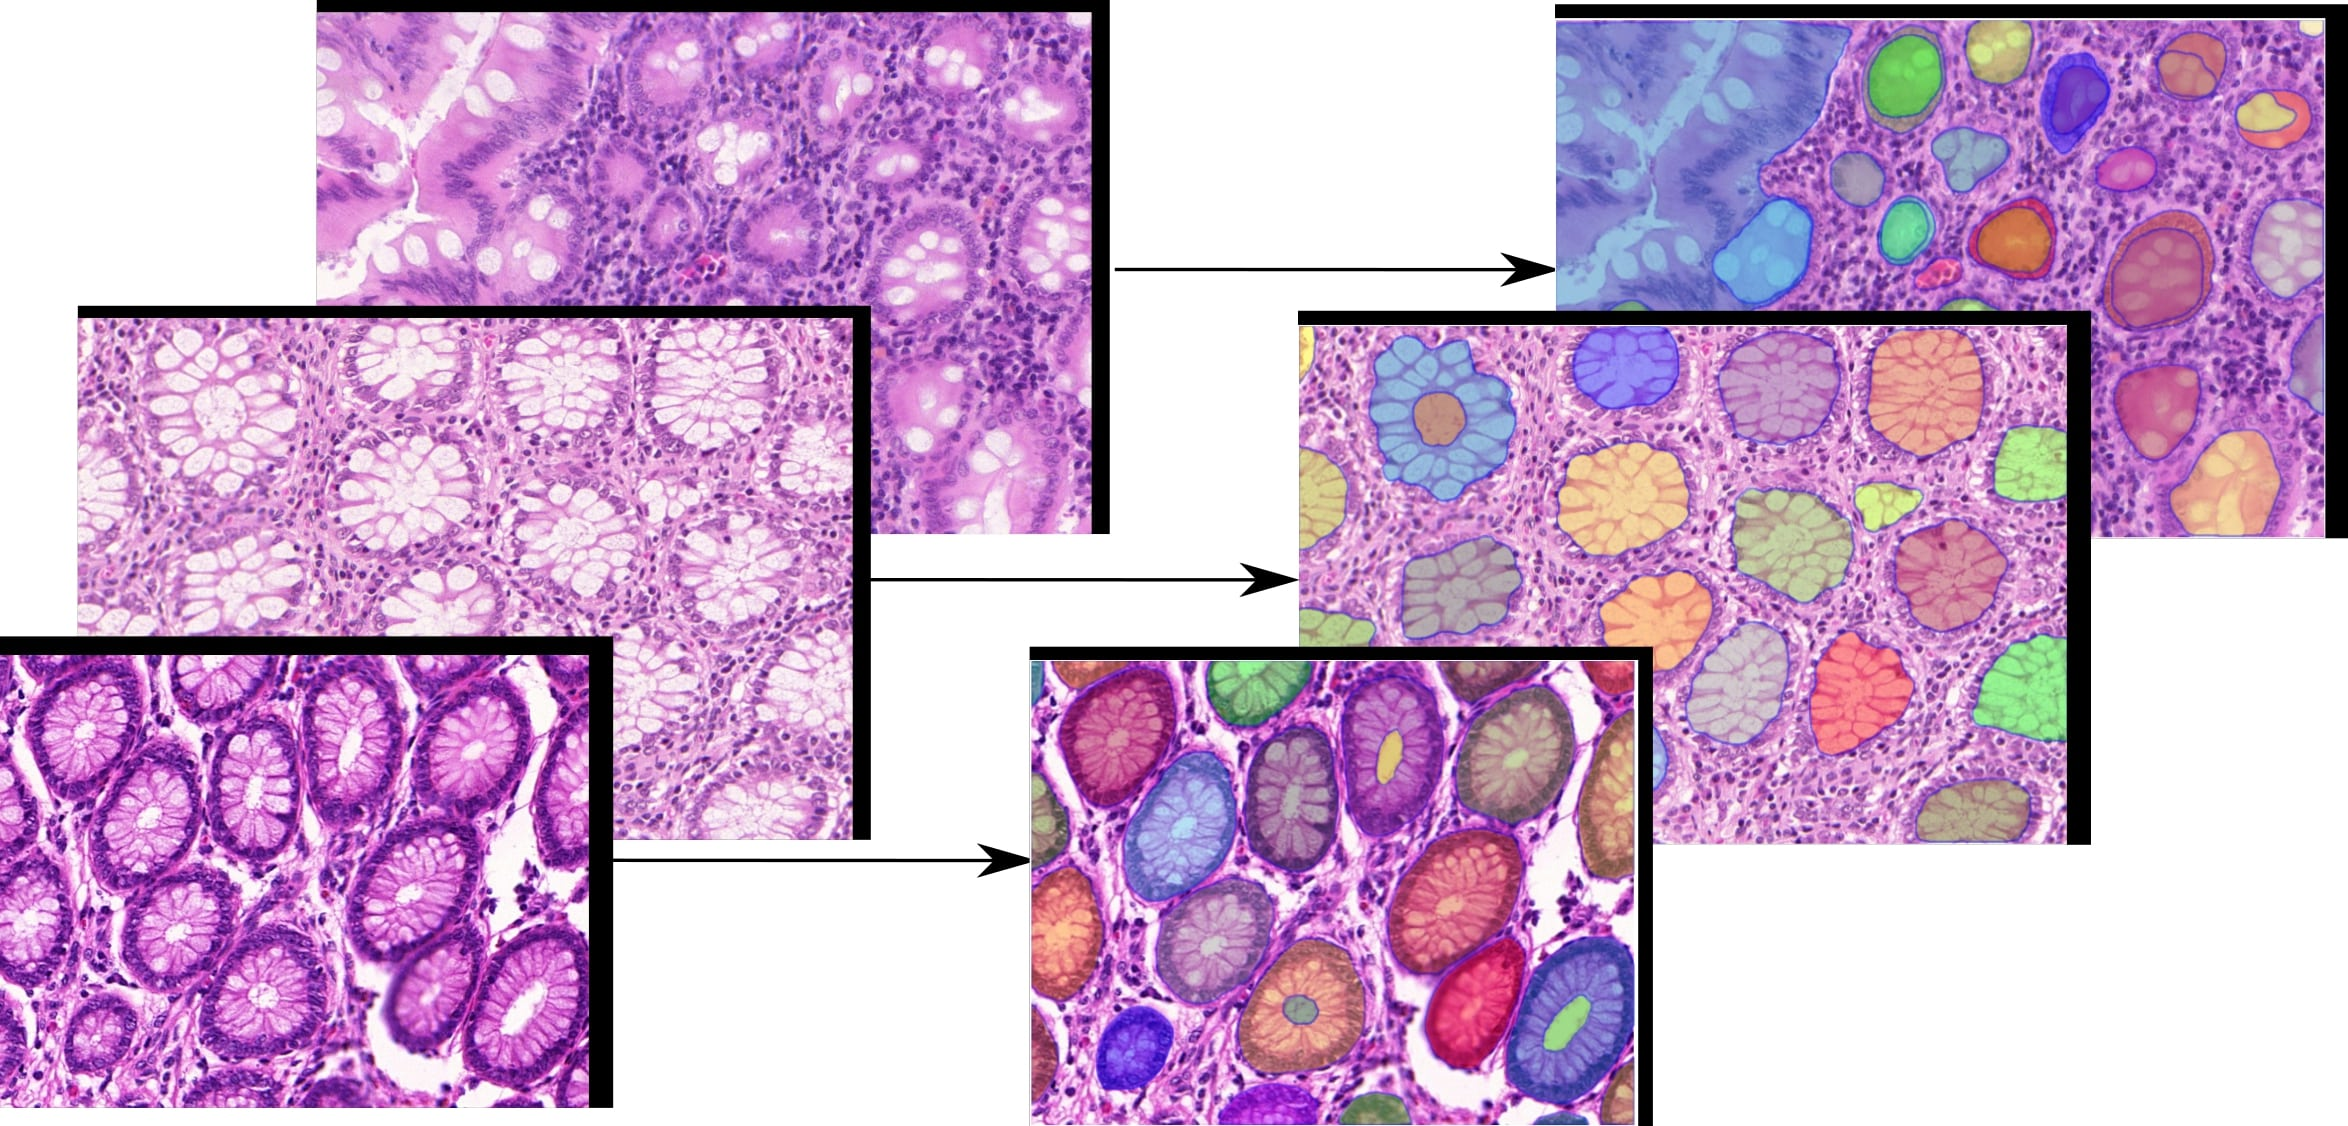
\includegraphics[width=0.6\textwidth]{labelled.jpg}
   \caption{Imágenes histopatológicas anotadas por expertos para guiar el aprendizaje (aprendizaje supervisado). En el caso particular de imágenes histopatológicas es poco frecuente que se tenga acceso a numerosas imágenes anotadas.}
    \label{fig:labelled}
\end{figure}

\paragraph{Aprendizaje no supervisado:}

En contraposición, el aprendizaje de máquina no supervisado se utiliza cuando la información no está clasificada ni etiquetada \cite{chatterjee_machine_2021}, ya que, el proceso de etiquetación de datos es costoso y complejo: estimaciones realizadas por estudios enfocados en patología digital revelan que el tiempo para la anotación de WSI en tareas generales de patología puede variar entre 45 segundos a 360 minutos dependiendo de la complejidad de la tarea\cite{lindman_annotations_2019}. Además, el enfoque no supervisado tiene la ventaja que permite explorar la forma en la que se organizan los datos, permitiendo encontrar estructuras ocultas en conjuntos de datos sin etiquetar \cite{chatterjee_machine_2021}. Siendo así que en este caso el algoritmo no busca la salida correcta, ya que no se cuenta con etiquetas. Este tipo de algoritmos permite extraer información valiosa\cite{chatterjee_machine_2021}, como por ejemplo con los algoritmos de agrupación (ver Figura \ref{fig:clustering}), asociación y los de reducción de dimensionalidad, de esta manera se busca encontrar similitudes entre los datos permitiendo crear agrupaciones y categorías o encontrar representaciones de baja dimensionalidad que sirvan para reconstruir los datos de entrada con poca información.

\begin{figure}
\centering
\subcaptionbox{Cluster A}{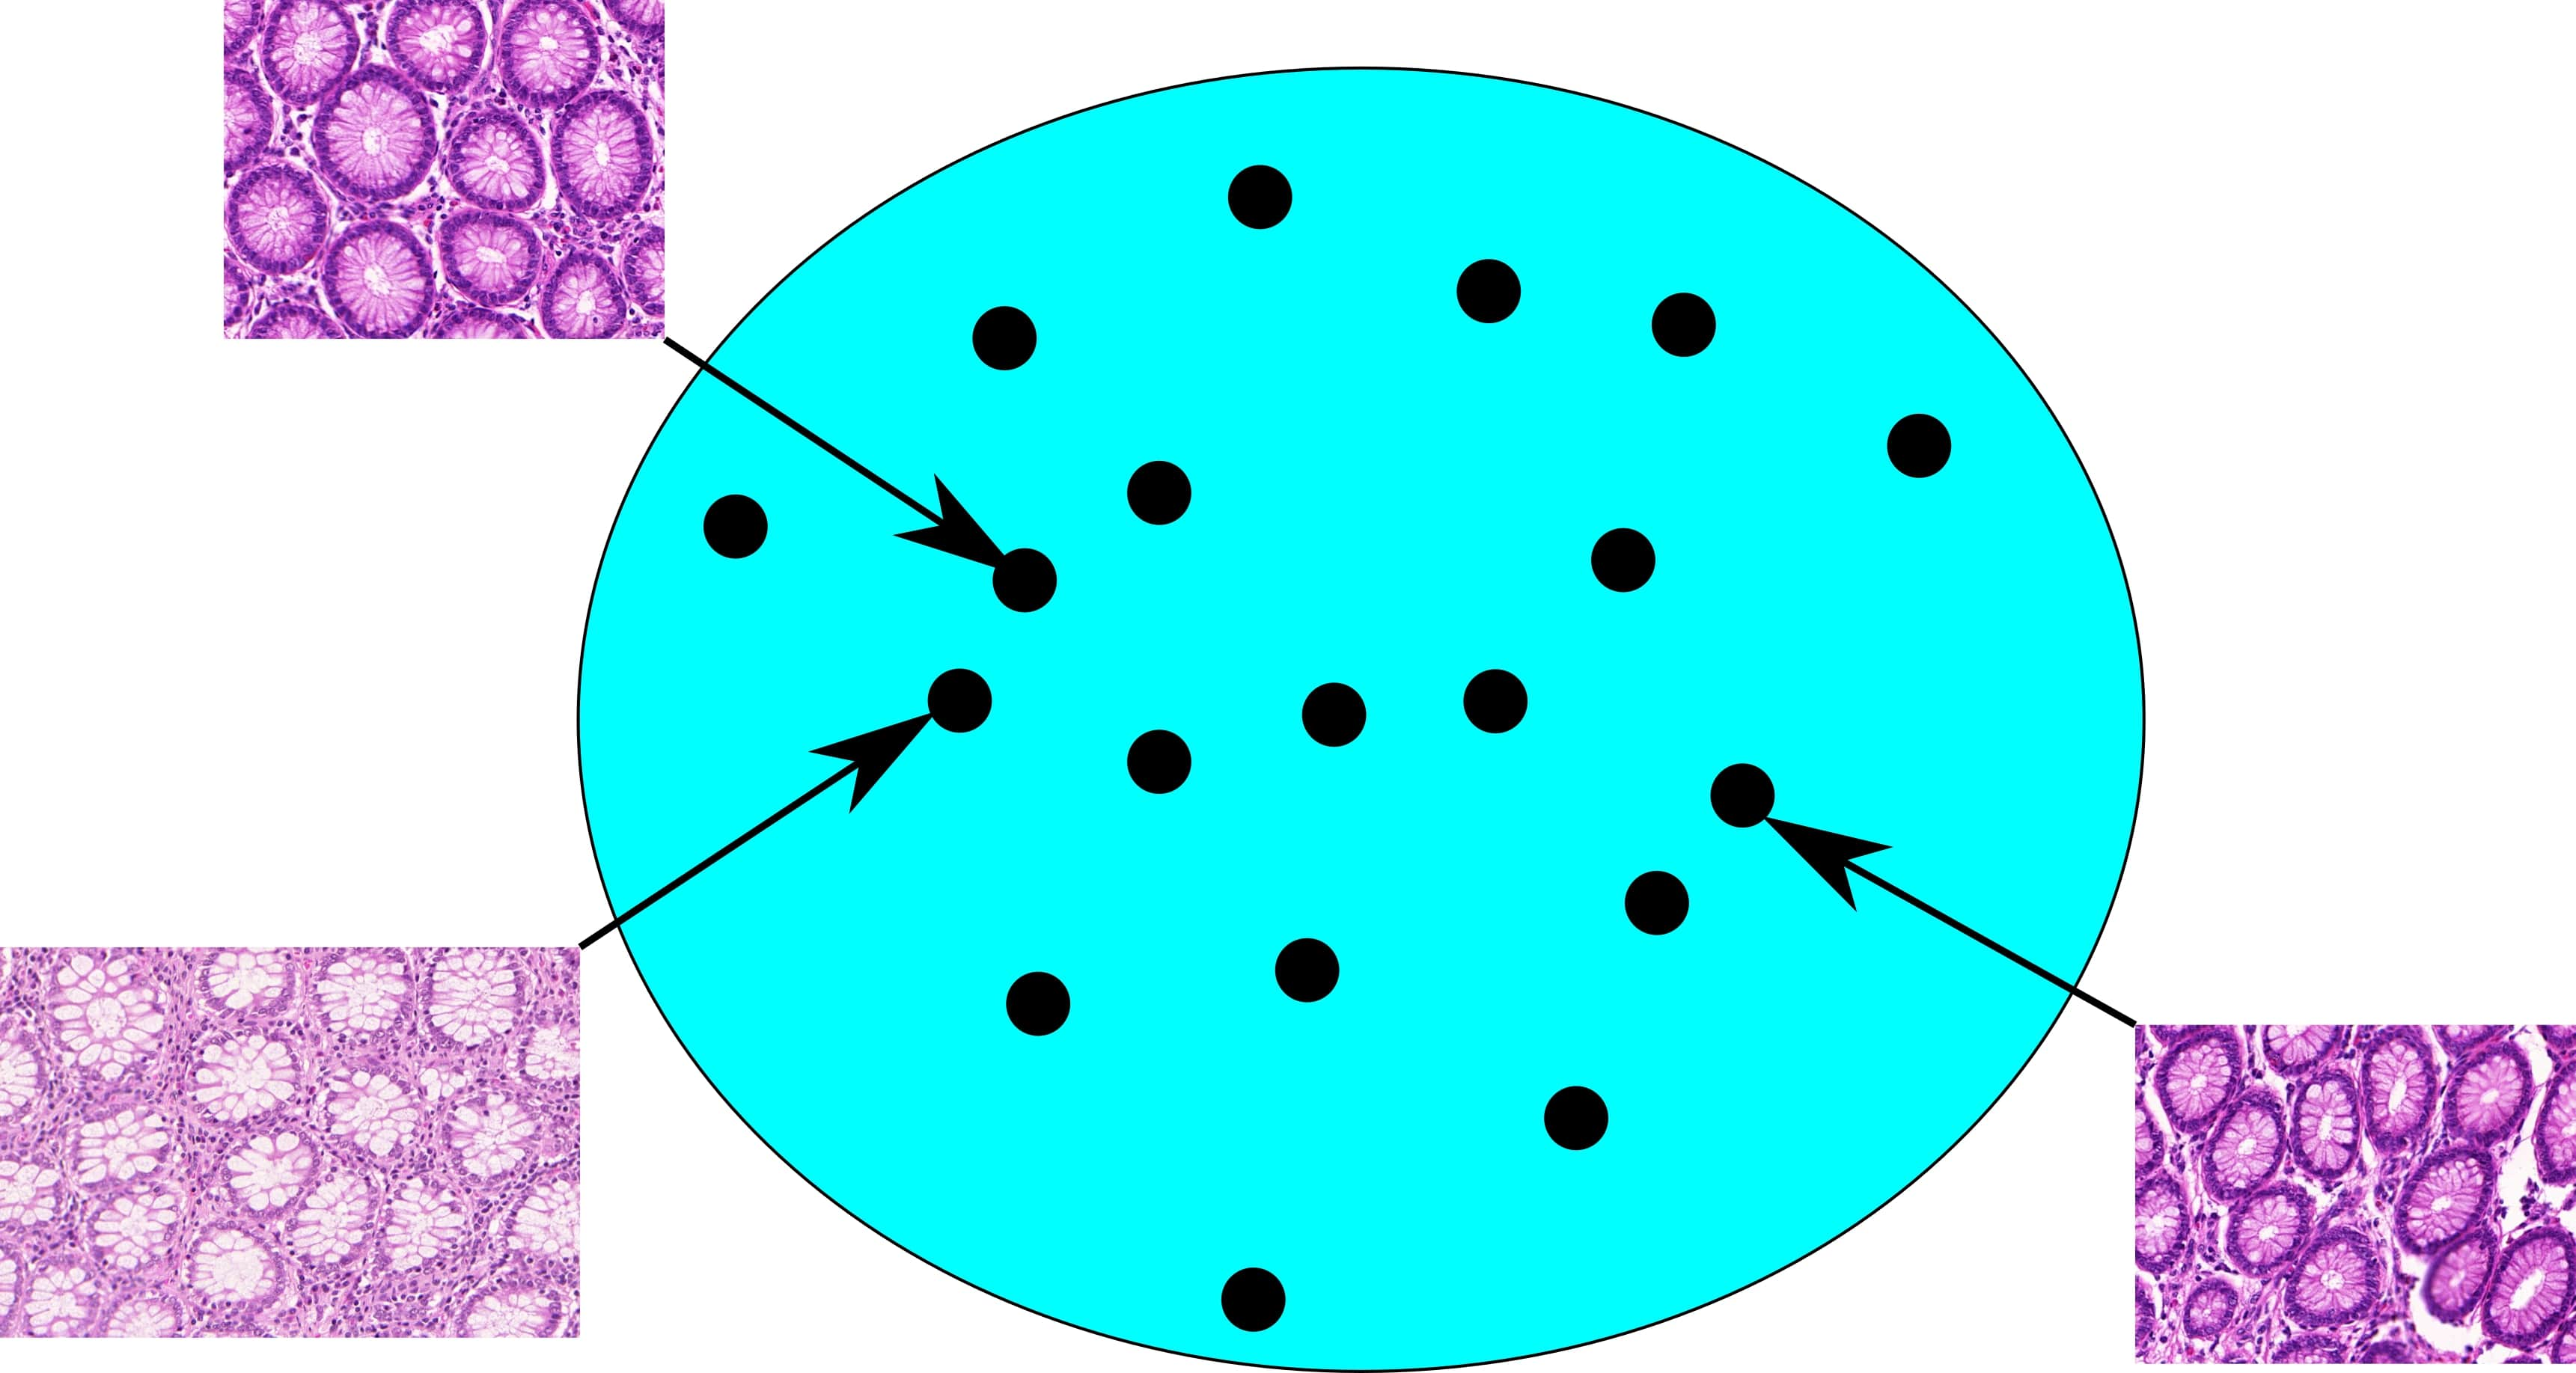
\includegraphics[width=0.55\textwidth]{cluster_A.jpg}}%
\hfill
\subcaptionbox{Cluster B}{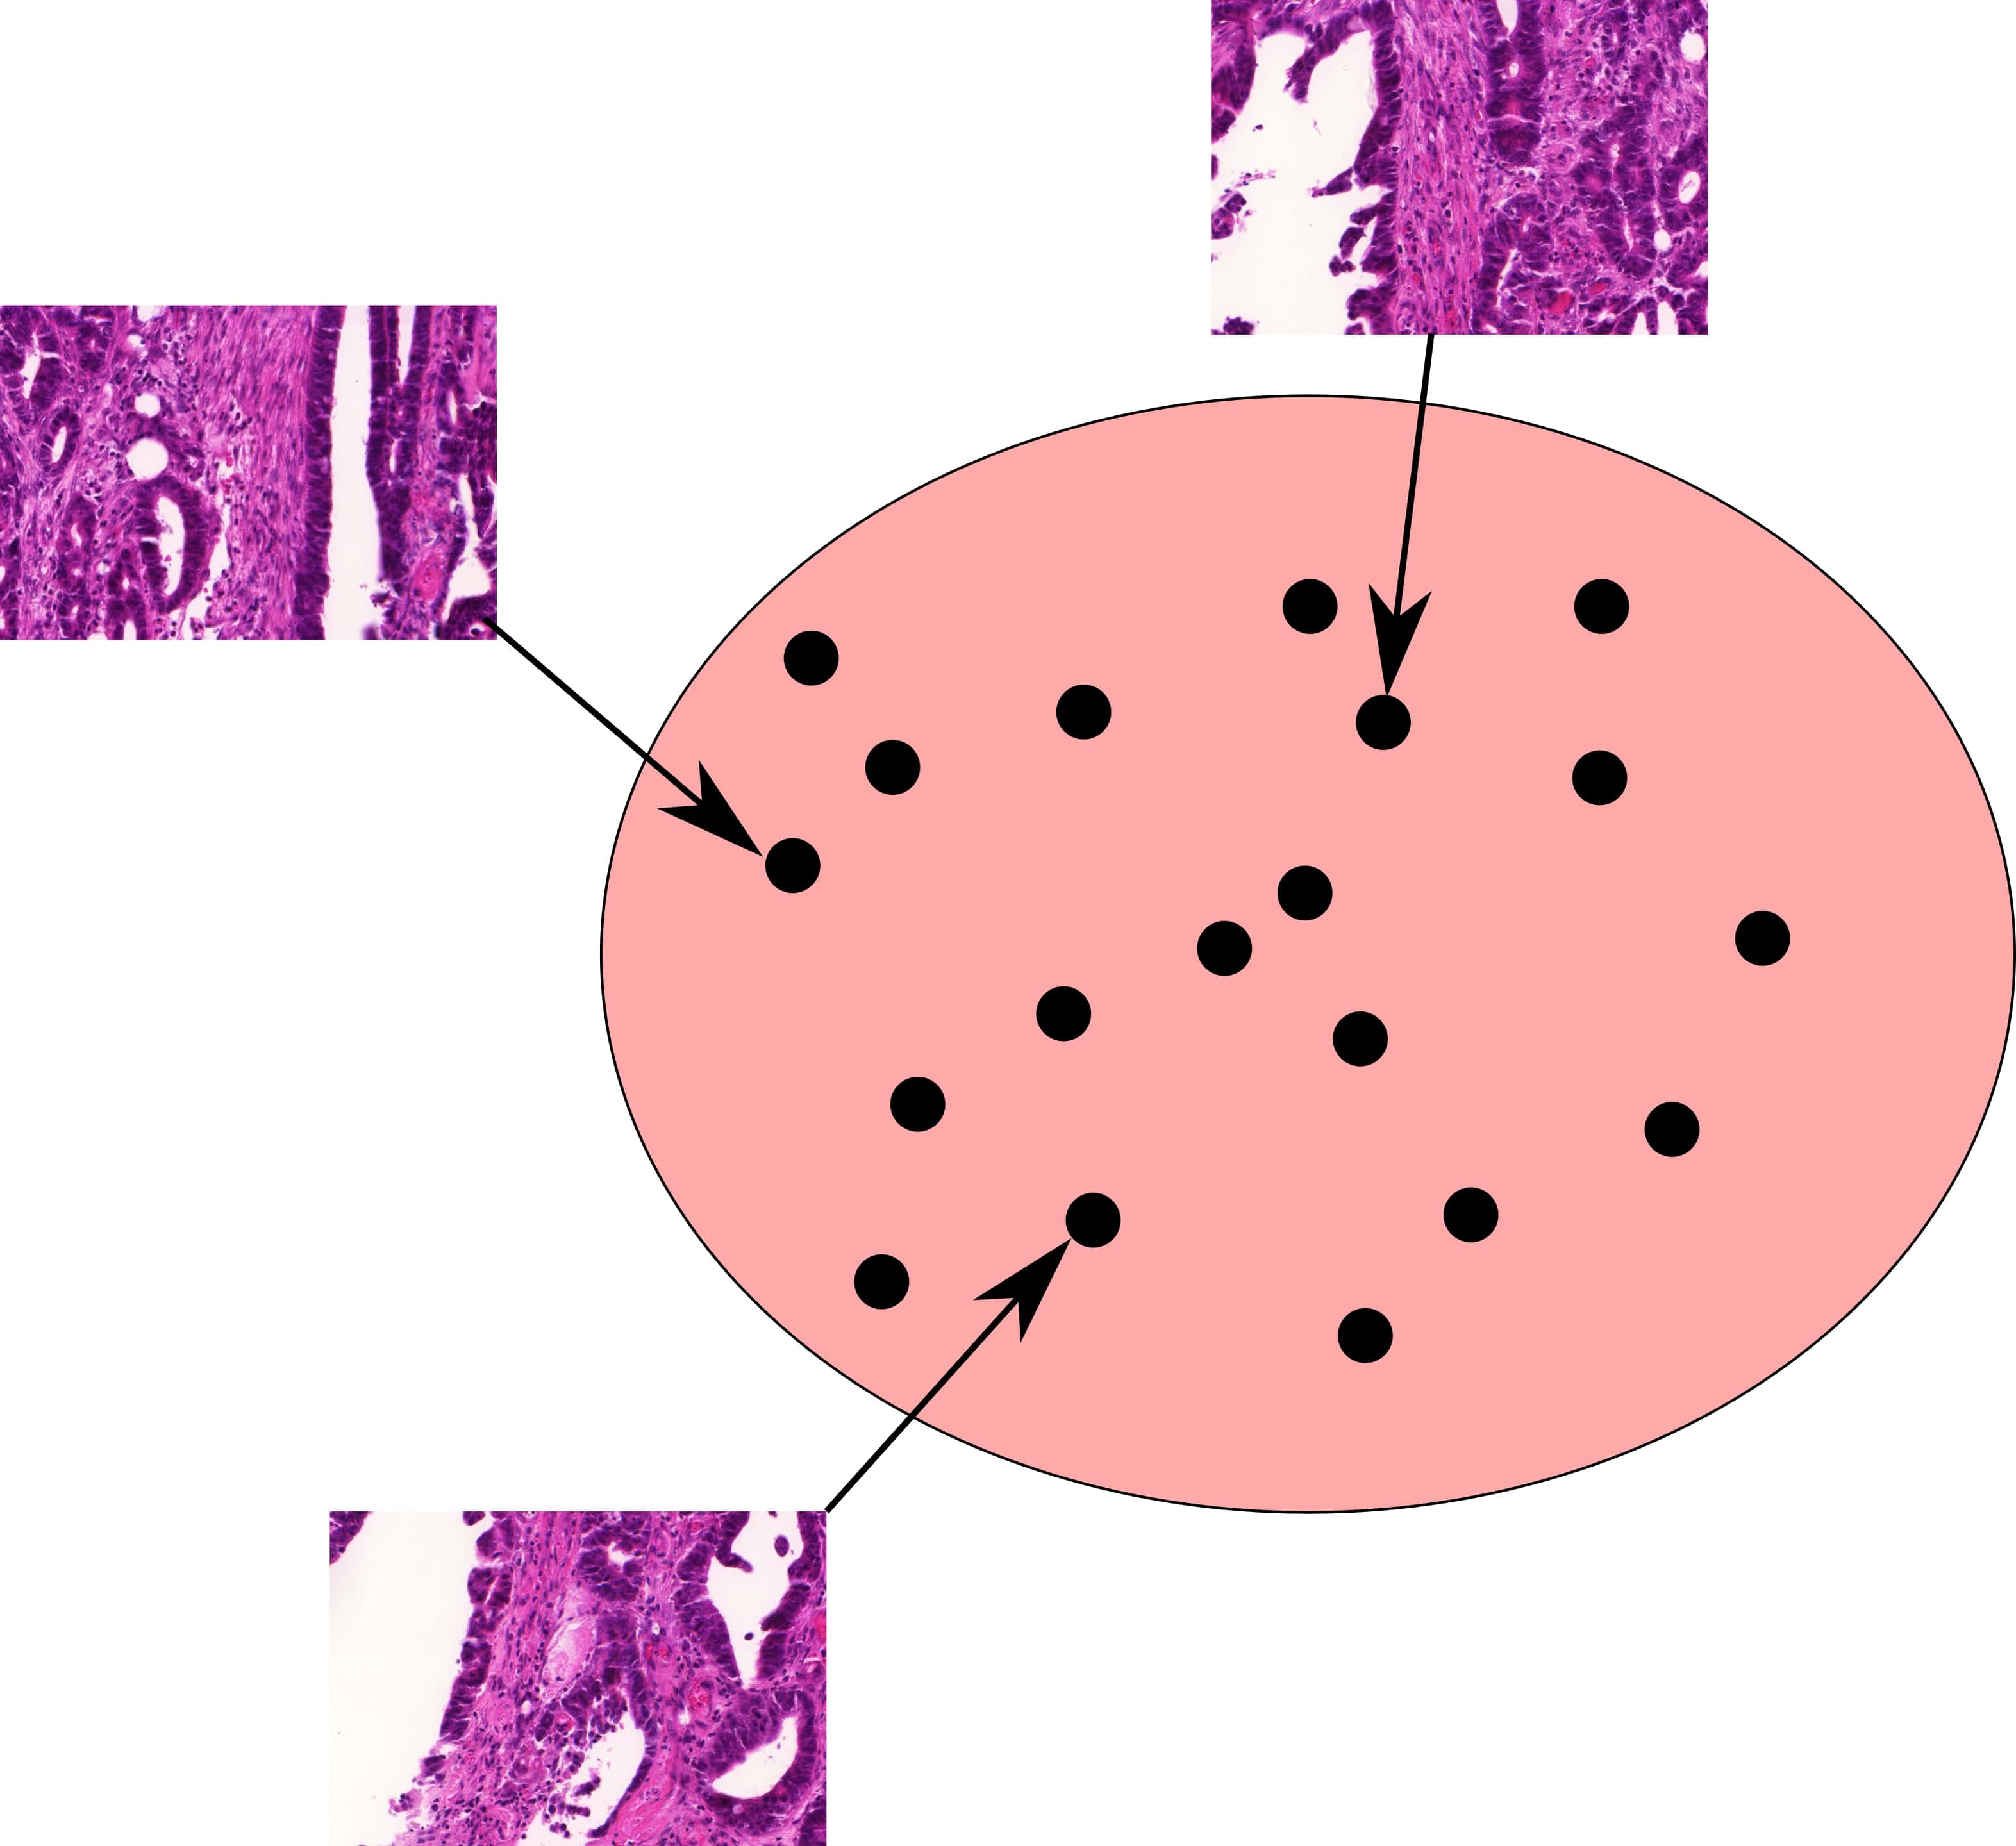
\includegraphics[width=0.45\textwidth]{cluster_B.jpg}}%
\hfill
\caption{Agrupación de imágenes similares como una forma de aprendizaje no supervisado.}
\label{fig:clustering}
\end{figure}

%\begin{figure}[h!]
%    \centering
%    
\includegraphics[width=0.4\textwidth]{unlabelled.jpg}
%   \caption{Un caso común en muchos hospitales y laboratorios es el acceso a muchas imágenes histopatológicas que no tienen anotaciones.}
%   \label{fig:unlabelled}
%\end{figure}


\paragraph{Aprendizaje semi-supervisado:}

Un tercer tipo de aprendizaje de maquina intermedio entre los dos anteriores es el de aprendizaje de máquina semi-supervisado, en los casos donde hay muchos datos no anotados y pocos datos anotados (ver Figura \ref{fig:semi-supervised}. Este procedimiento es usado en casos en los cuales los datos son variados porque combinan datos etiquetados y no etiquetados para el entrenamiento de maquina permitiendo el uso del aprendizaje supervisado y el no supervisado dependiendo de las características especificas de los datos en cuestión \cite{chatterjee_machine_2021}. Por ejemplo, se usan datos que presentan o pocas etiquetas o sin etiquetar \cite{chatterjee_machine_2021}. Por consiguiente, este tipo de aprendizaje de máquina es implementado para mejorar significativamente la precisión del modelo en vez de limitarse al uso de pocos datos etiquetados \cite{chatterjee_machine_2021}.

\begin{figure}[h!]
    \centering
    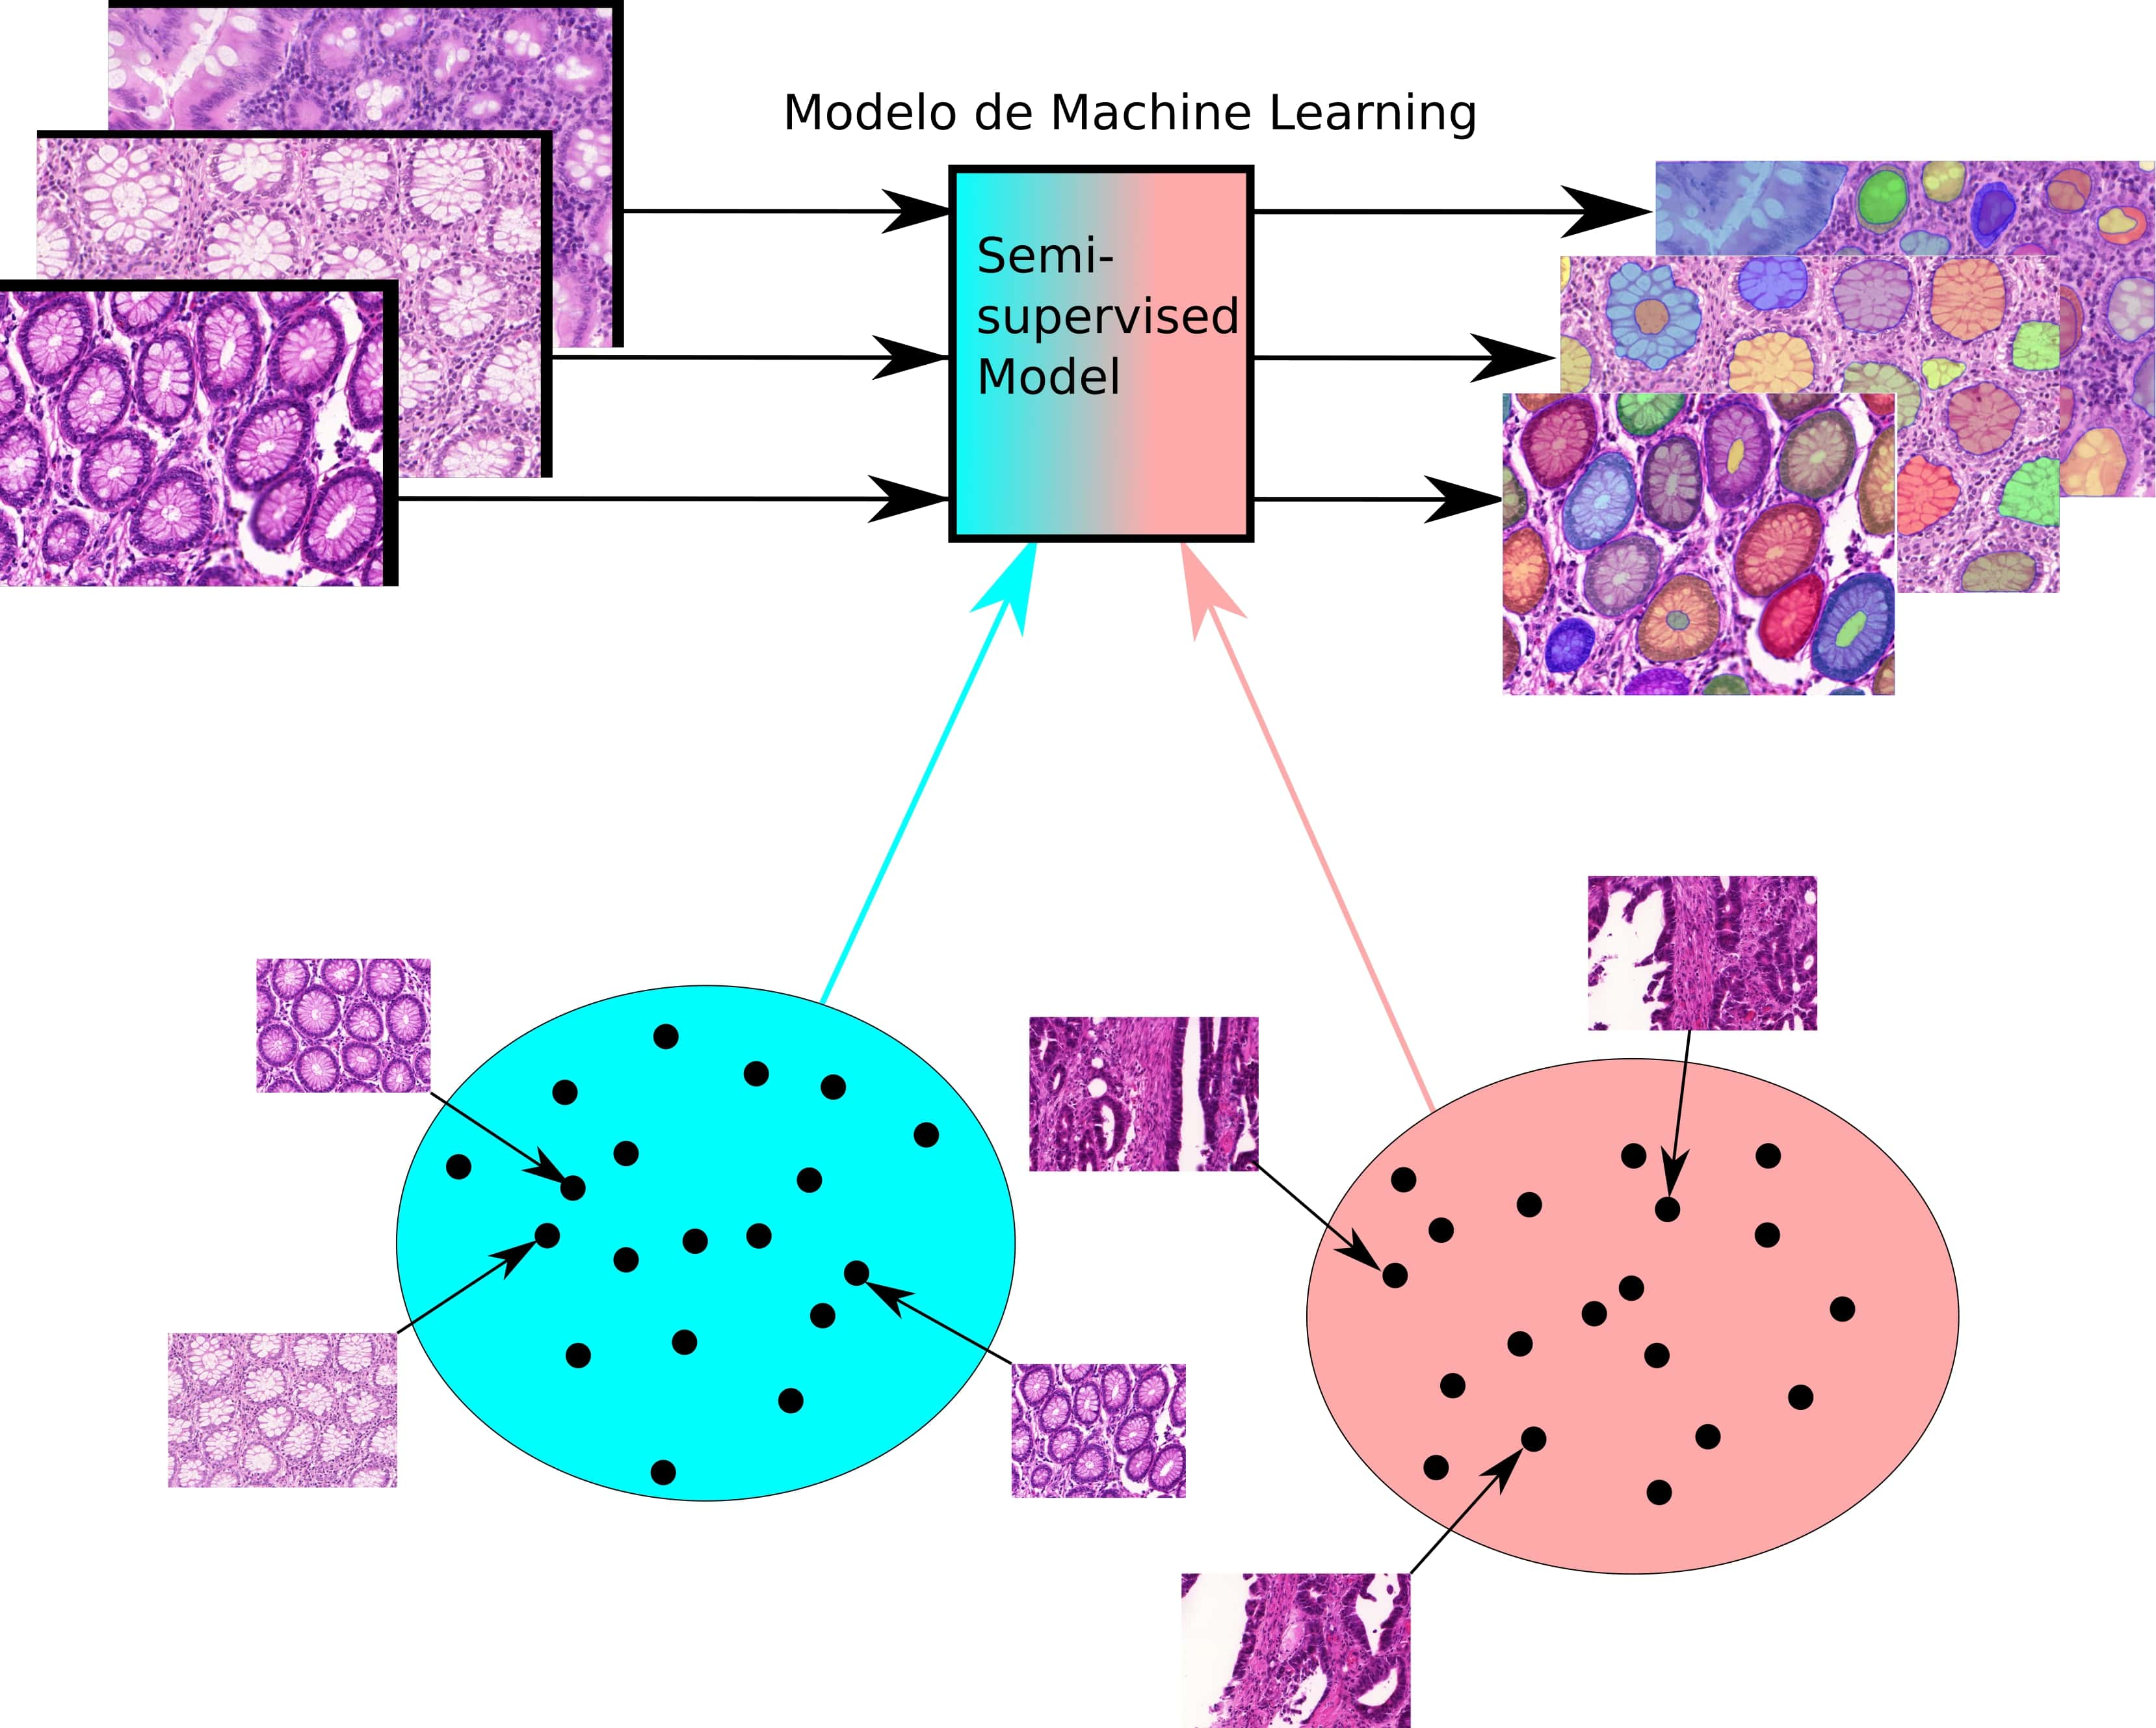
\includegraphics[width=\textwidth]{semi_supervised_model.jpg}
    \caption{Se muestra un ejemplo de modelo de aprendizaje no supervisado, donde la tarea del modelo es aprender a segmentar de células de manera supervisada (con imágenes anotadas por expertos), pero el modelo se ayuda de un proceso no supervisado de clustering para mejorar su predicción (con imágenes no anotadas). Es frecuente en el contexto de la patología digital tener acceso a una cantidad numerosa de imágenes no anotadas y una baja cantidad de imágenes anotadas, por lo que un modelo semi-supervisado podría ser ideal.}
    \label{fig:semi-supervised}
\end{figure}
%\begin{figure}[h!]
%    \centering
%    
\includegraphics[width=0.6\textwidth]{encoder_decoder.jpg}
%    \caption{Una posible forma de hacer aprendizaje semi-supervisado es primero entrenar un modelo que aprenda a ``comprimir" la información (que aprenda a representar la entrada en un espacio latente de muy baja dimensionalidad), en este ejemplo se puede ver una arquitectura de codificador-decodificador, donde el codificador aprende a comprimir la información y el decodificador aprende a descomprimirla, en el proceso encontrando un espacio de baja dimensionalidad que pueda representar la imagen en su totalidad, cabe notar que entonces el input y el output es la misma imagen, por lo que el aprendizaje depende de las transformaciones que el modelo haga internamente. Posterior a este paso no supervisado, se procede con el paso supervisado: en este ejemplo se muestra como se puede tomar el codificador y las representaciones de baja dimensionalidad que genera y se puede cambiar el decodificador. Esto busca que el modelo solo deba entrenar un decodificador en vez de un modelo entero, además, como el decodificador toma representaciones de baja dimensionalidad, en general va a necesitar muchos menos parámetros, por lo que incluso con pocos datos anotados se puede obtener buenos resultados.}
%    \label{fig:encoder_decoder}
%\end{figure}

%Un ejemplo de lo anterior puede observarse en el caso de un hospital, ya que al mismo tiempo que este genera muchas imágenes médicas, es improbable que estas imágenes puedan ser implementadas con un enfoque supervisado debido a que no están etiquetadas ni segmentadas. Ya que para poder llevar a cabo este tipo de entrenamiento supervisado, se requeriría que especialistas en el área médica correspondiente se encargaran de revisar imagen por imagen - un proceso sumamente costoso y dilatado en tiempo. En vez de esto, con la ayuda del aprendizaje semi-supervisado es posible etiquetar una cantidad limitada de datos y complementar el entrenamiento con todos los otros datos sin etiquetar haciéndolo viable en términos de recursos tanto económicos como de tiempo.

\section{Redes neuronales profundas}

Una red neuronal en el contexto del aprendizaje automático es un modelo computacional inspirado en la estructura y funcionamiento de las neuronas interconectadas del cerebro humano, en medida que es un tipo de algoritmo que consta de capas de nodos o neuronas conectados de manera jerárquica. Como su nombre indica, las neuronas son los componentes básicos de una red neuronal. Cada neurona procesa las señales de entrada y sus salidas se envía a la siguiente capa de neuronas. Las conexiones internas entre neuronas tienen un peso que determina cuánto influye cada señal de entrada. Después de multiplicar la entrada por el peso, se aplica una función de activación a la suma ponderada de las entradas. Las funciones de activación más comunes son la sigmoide, la tangente hiperbólica (tanh), la Unidad Lineal Rectificada (RELU) y la función softmax. Para una representación gráfica de una red neuronal, ver la Figura \ref{fig:deep_nets}.
\begin{figure}[h!]
    \centering
    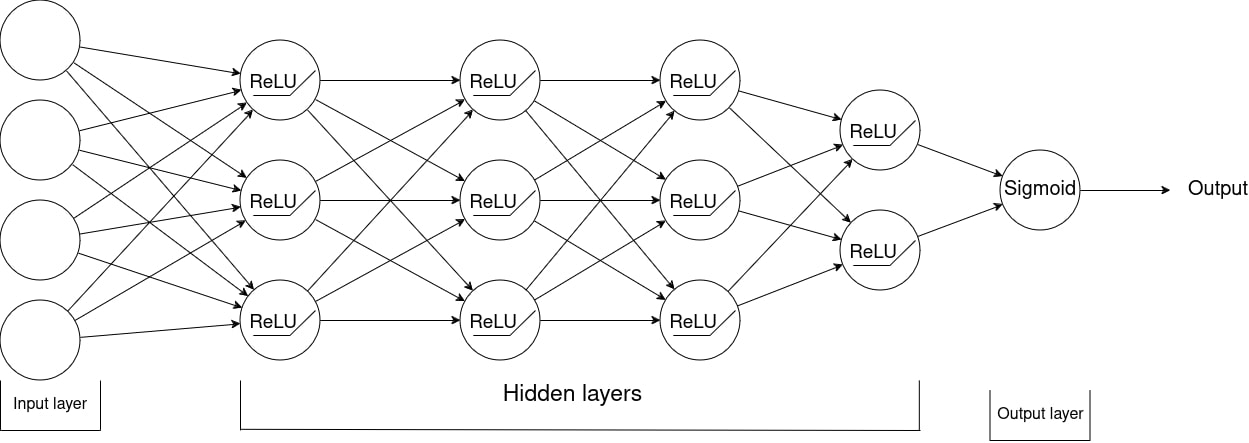
\includegraphics[width=0.9\textwidth]{neural_nets.drawio.jpg}
    \caption{Ejemplo de una red neuronal profunda: la capa de entrada recibe 4 valores, luego hay 4 capas ocultas, donde cada neurona aplica una función ReLU. Finalmente la capa de salida aplica una función sigmoide y entrega un valor.}
    \label{fig:deep_nets}
\end{figure}

Se les llama profundas a estas redes debido a que las neuronas se organizan en capas. Normalmente, una red neuronal consta de una capa de entrada, una o más capas ocultas apiladas en sucesión y una capa de salida. La capa de entrada recibe los datos iniciales, las capas ocultas los procesan y la capa de salida produce el resultado final. Durante la fase de entrenamiento, la red neuronal recibe datos de entrada, los pasa a través de las capas mediante un proceso llamado feedforward, calcula la salida y luego la compara con la salida esperada. Luego utiliza una técnica llamada backpropagation para ajustar los pesos y sesgos con el fin de minimizar la diferencia entre los resultados previstos y reales. Las redes neuronales aprenden de ejemplos ajustando sus pesos y sesgos mediante algoritmos de entrenamiento como el gradiente descendiente, donde la red intenta minimizar una función de costo o pérdida que mide la diferencia entre los resultados previstos y reales.
%\\
%\\
%Gracias a esto, las redes neuronales son capaces de aprender patrones y relaciones complejos a partir de datos, lo que las convierte en herramientas poderosas para diversas tareas de aprendizaje automático, como clasificación, regresión, reconocimiento de patrones y más. Hasta la fecha, las redes neuronales se han implementado con éxito en diversas áreas de aplicación, entre ellas - el reconocimiento de imágenes y voz, el procesamiento del lenguaje natural, la robótica y las finanzas. Las redes actuales se caracterizan por su profundidad, pues suelen tener numerosas capas, contando con millones de parámetros, lo que las hace computacionalmente costosas de entrenar ya que necesiten una cantidad formidable de datos de entrenamiento. Aunque al aumentar la cantidad de capas hace que sea más complejo el entrenamiento de la red neuronal, estas mismas capas ocultas permiten que las redes neuronales profundas aprendan representaciones complejas de datos extrayendo progresivamente características de nivel superior a partir de las entradas sin siquiera tener que limpiar datos.
%\\
%\\
%De esta manera, las redes neuronales profundas han sido fundamentales para avanzar en el campo de la inteligencia artificial, logrando un rendimiento de vanguardia en diversos campos de aplicación, en particular - la visión por computadora, el procesamiento del lenguaje natural, el reconocimiento de voz y el aprendizaje por refuerzo. Ejemplos de arquitecturas de redes neuronales profundas incluyen redes neuronales convolucionales, para el reconocimiento de imágenes, redes neuronales recurrentes, para el procesamiento secuencial de datos y transformadores para tareas de procesamiento del lenguaje natural.
\\
\\
De particular interés para este proyecto son las redes neuronales convolucionales (Convolutional Neural Network, CNN), las cuales son un tipo especializado de red neuronal profunda diseñada para procesar datos con una estructura geométrica en forma de cuadrícula, como imágenes o secuencias de audio. Las CNN son particularmente efectivas en tareas de visión por computadora, pero también se han aplicado con éxito a otros campos de aplicación tales como el procesamiento del lenguaje natural y el análisis de audio. Las CNN están inspiradas en la organización de la corteza visual animal, donde las neuronas responden a regiones superpuestas en el campo visual. Por analogía, la operación de convolución es una forma de mezclar dos funciones, se puede visualizar como voltear y luego deslizar una función sobre la otra, anotando el resultado en cada punto. Un ejemplo común consiste en aplicar un filtro a una imagen, como se puede ver en la Figura ~\ref{fig:convolution}.
\\
\begin{figure}[h!]
    \centering
    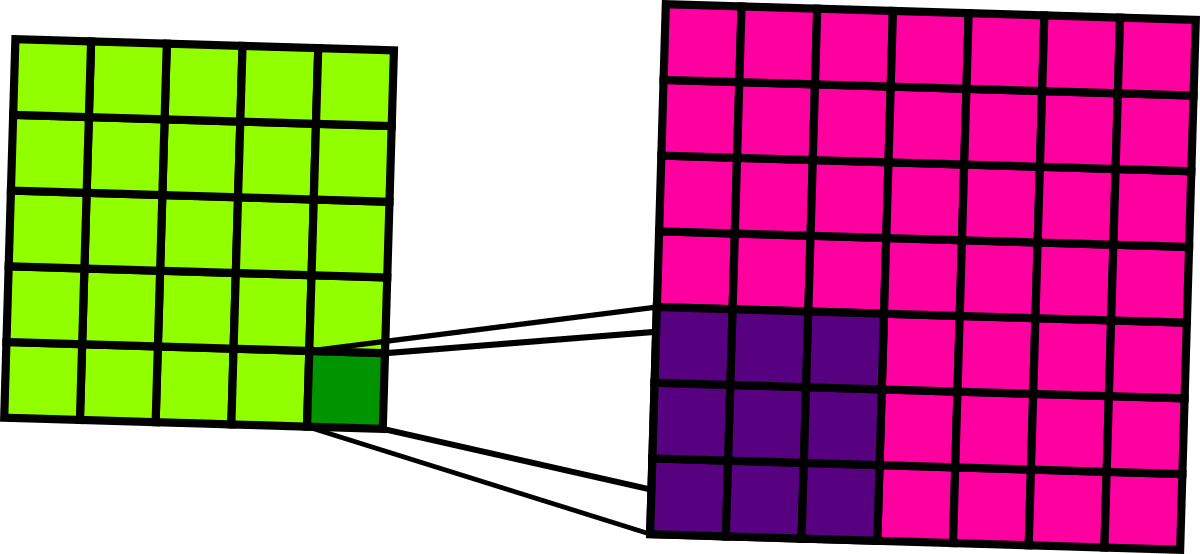
\includegraphics[width=0.6\textwidth]{convolution_classical.png}
    \caption{Ejemplo de convolución discreta para un filtro que se desliza sobre la grilla magenta. La función del filtro la transforma a otro valor (color verde). Se puede ver que el proceso es local: solo se toman elementos que conforman un vecindario en la grilla para generar el resultado.}
\label{fig:convolution}
\end{figure}


En general la convolución de dos funciones $f,g \rightarrow \mathbb{R}$ se escribe como $(f*g)(x) \rightarrow \mathbb{R}$ que es otra función  y se define como la integral del producto de ambas funciones después de desplazar una de ellas una distancia $t$ de la siguiente manera:

\begin{equation}
(f * g)(x) = \int_{-\infty}^{\infty} f(y)g(x-t)dt
\end{equation}


El caso discreto es similar al caso continuo pero ahora las funciones  $f[m],g[m] \rightarrow \mathbb{Z}$  reciben valores discretos y la integral es reemplazada por una sumatoria y, así mismo, el desplazamiento sobre la variable $[n]$ también es discreto, define como:
\begin{equation}
(f * g)[n] = \sum_{m=-\infty}^{\infty} f[m]g[n-m]
\end{equation}

%Es así que las CNN son de particular interés para el procesamiento de imágenes ya que las imágenes contienen información geométrica debido a que cada pixel contiene una alta correlación con píxeles adyacentes y baja con los píxeles distantes. Las CNN pueden explotar esta información para mejorar su rendimiento usando menos parámetros, en particular utilizan una arquitectura jerárquica que consta de capas convolucionales, capas de agrupación y capas completamente conectadas. El proceso que usan las capas convolucionales consiste en la aplicación de filtros aprendibles (núcleos o kernels) a través de los datos de entrada para extraer características locales como bordes, texturas y patrones. Es así como estas capas aprenden a detectar características cada vez más complejas a medida que la red se vuelve más profunda, produciendo una jerarquía espacial de características.

Es importante tener en cuenta que las CNN, al usar filtros, son inherentemente equivariantes a la traslación, lo que implica que estas pueden reconocer patrones independientemente de su posición en la entrada. Esta propiedad se logra mediante capas convolucionales, que comparten pesos entre posiciones espaciales. Como resultado, las CNN no son afectadas por las traslaciones y pueden identificar eficazmente objetos en imágenes independientemente de su ubicación, una propiedad altamente deseable en datos estructurados, como es el caso de las imágenes. Debido al a priori que se tiene sobre la estructura geométrica de las imágenes, las CNN también pueden explotar el concepto de compartir parámetros, al que se aplica el mismo conjunto de pesos en diferentes ubicaciones espaciales. Esto reduce significativamente la cantidad de parámetros en la red, lo que la hace más eficiente desde el punto de vista computacional y más fácil de entrenar, especialmente cuando se trata de entradas de alta dimensión como imágenes.

%En añadidura a las capas convolucionales, también se usan capas de agrupación, las cuales se utilizan para reducir progresivamente las dimensiones espaciales de los mapas de características producidas por las capas convolucionales. La agrupación ayuda a capturar las características más destacadas y al mismo tiempo descarta detalles irrelevantes, lo que conduce a una mejor generalización que se traduce en una mayor eficiencia computacional.

%En suma, similar a otras redes neuronales profundas, las CNN aprenden representaciones jerárquicas de los datos de entrada. Sin embargo, en las CNN, estas representaciones capturan jerarquías espaciales de características de bajo nivel y nivel superior - entre las primeras se encuentran los bordes, mientras que las últimas incluyen partes de objetos y objetos completos.

%Es así como gracias a la explotación de esta información geométrica, las CNN han logrado un rendimiento de vanguardia en diversas tareas de visión por computadora, incluida la clasificación de imágenes, la detección de objetos, la segmentación de imágenes y la generación de imágenes.




\section{Redes neuronales convolucionales equivariantes}

Las redes neuronales convolucionales hacen uso de la simple observación según la cual las características geométricas locales en imágenes no cambian si son trasladadas, esto es, son equivariantes a la traslación, haciéndolas tremendamente eficientes para tareas de procesamiento de imágenes \cite{lim_what_2022}. Para ejemplificar, si se entrena una red convolucional en la segmentación de gatos y el gato en la imagen cambia de posición, la segmentación debe cambiar de la misma manera que la posición del gato, ya sea traslación, rotación o reflexión.

Con el fin de visualizar lo dicho anteriormente se presentan las siguientes imágenes de un gato y una sección de WSI que han sido transformadas de varias maneras, sin perder la información que contienen ver Figura \ref{fig:cat} (para mayor claridad los ejemplos siguientes se harán con imágenes naturales, como la del gato).
\begin{figure}[h!]
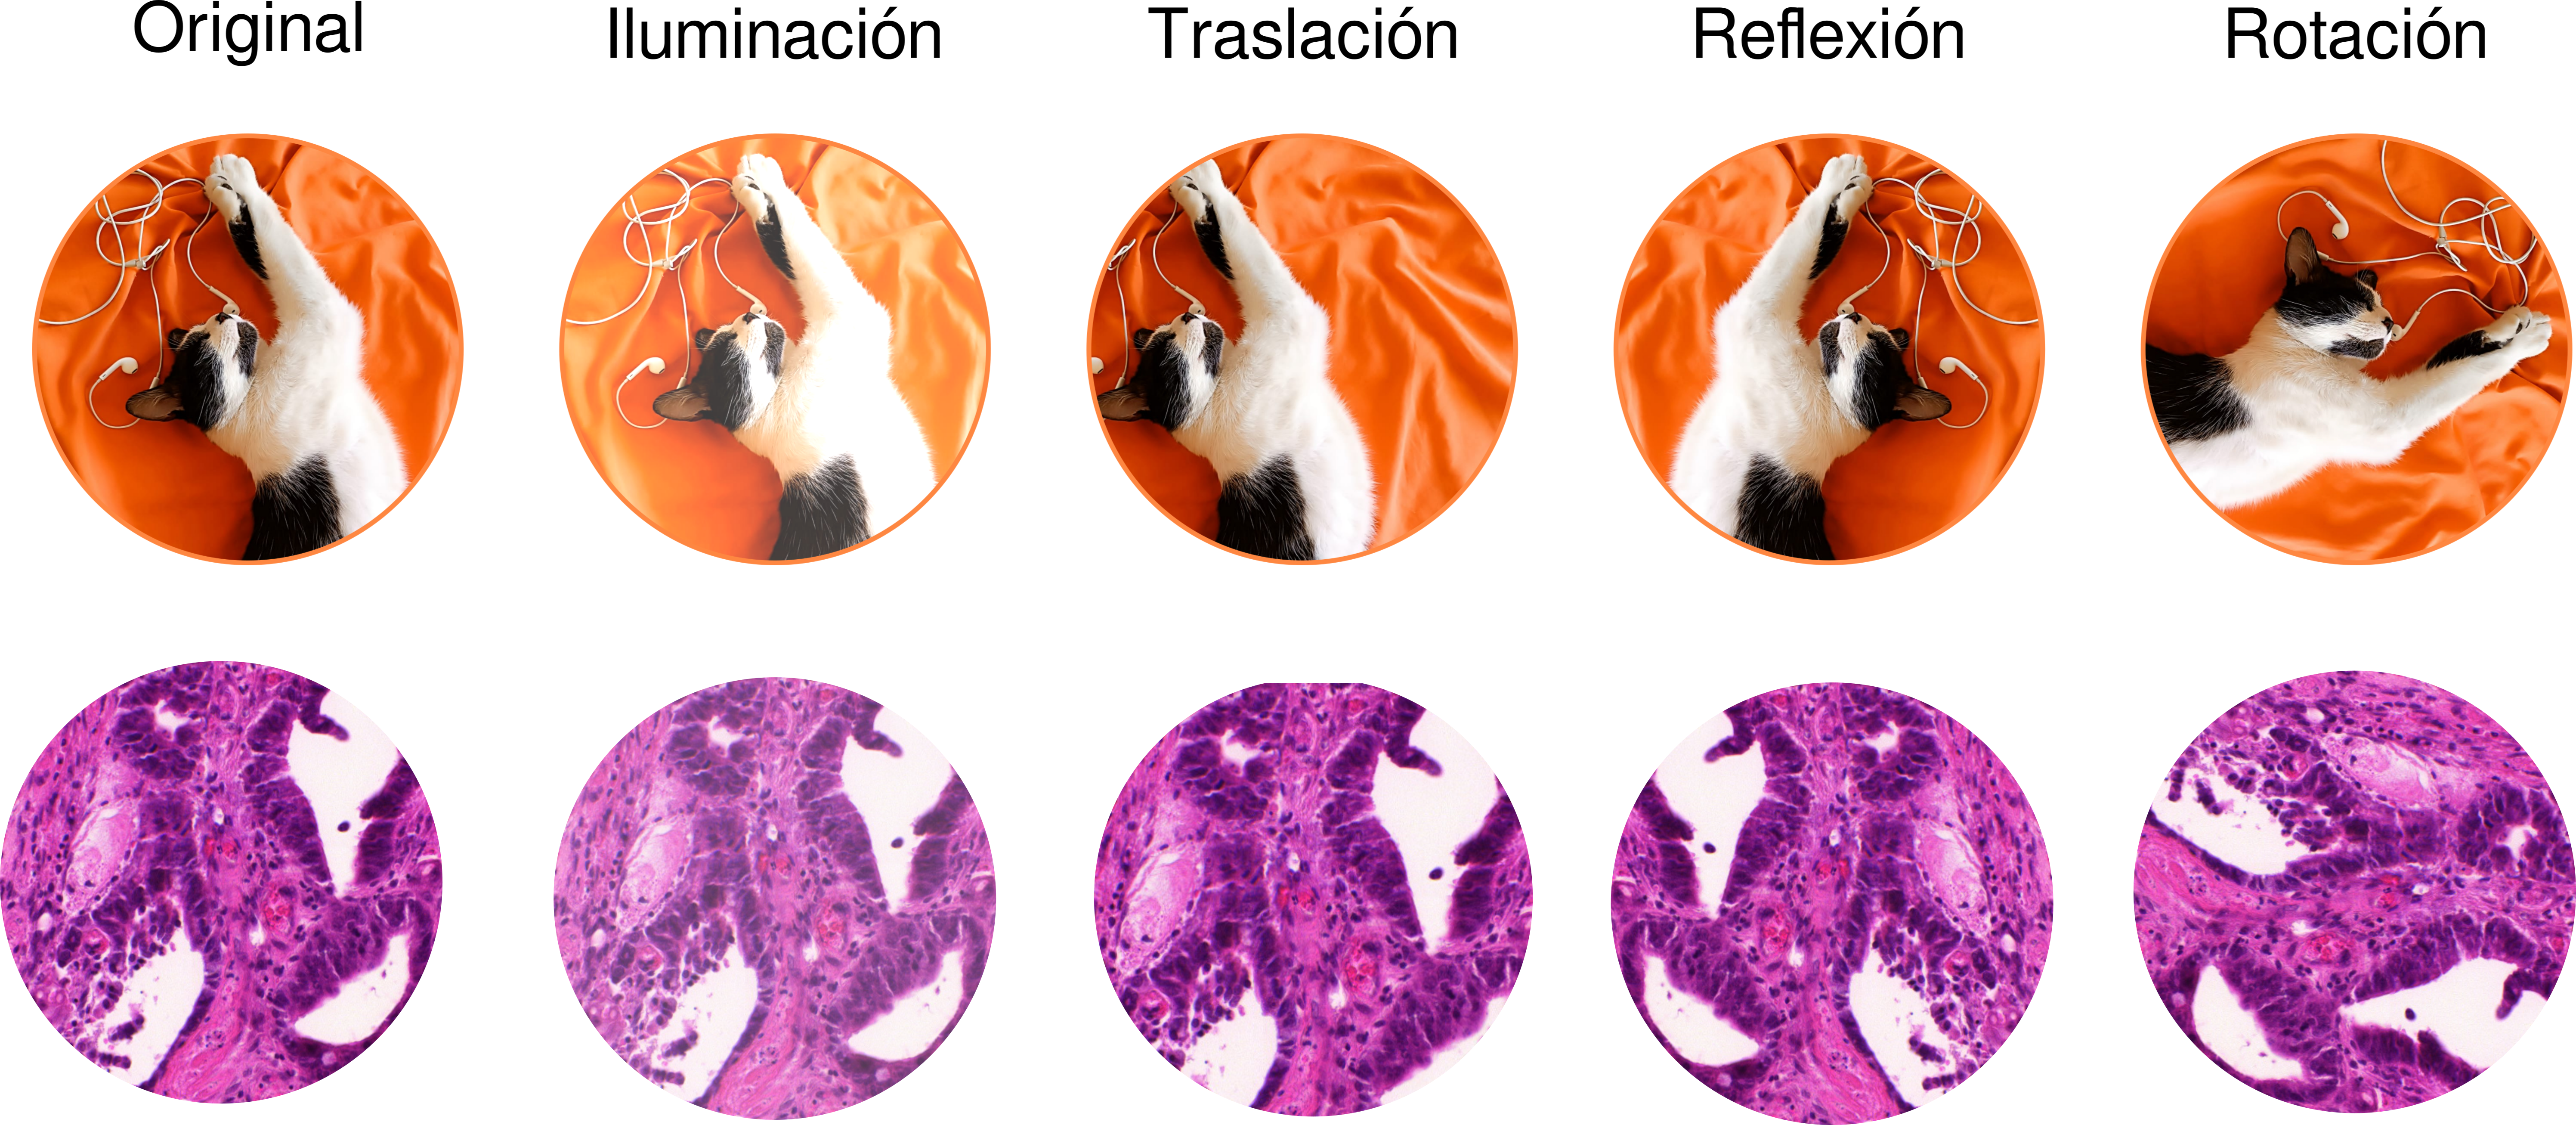
\includegraphics[width=1\textwidth]{transformaciones_gato_wsi.png}
\caption{Imagen sobre la que se aplican diferentes transformaciones.}
\label{fig:cat}
\end{figure}


Por analogía, una red neuronal debe poder clasificar o segmentar la imagen del gato sin importar la transformación que se realice. Ver Figura~\ref{fig:cat_segmentation}.

\begin{figure}[h!]
\centering
\subcaptionbox{Invarianza}{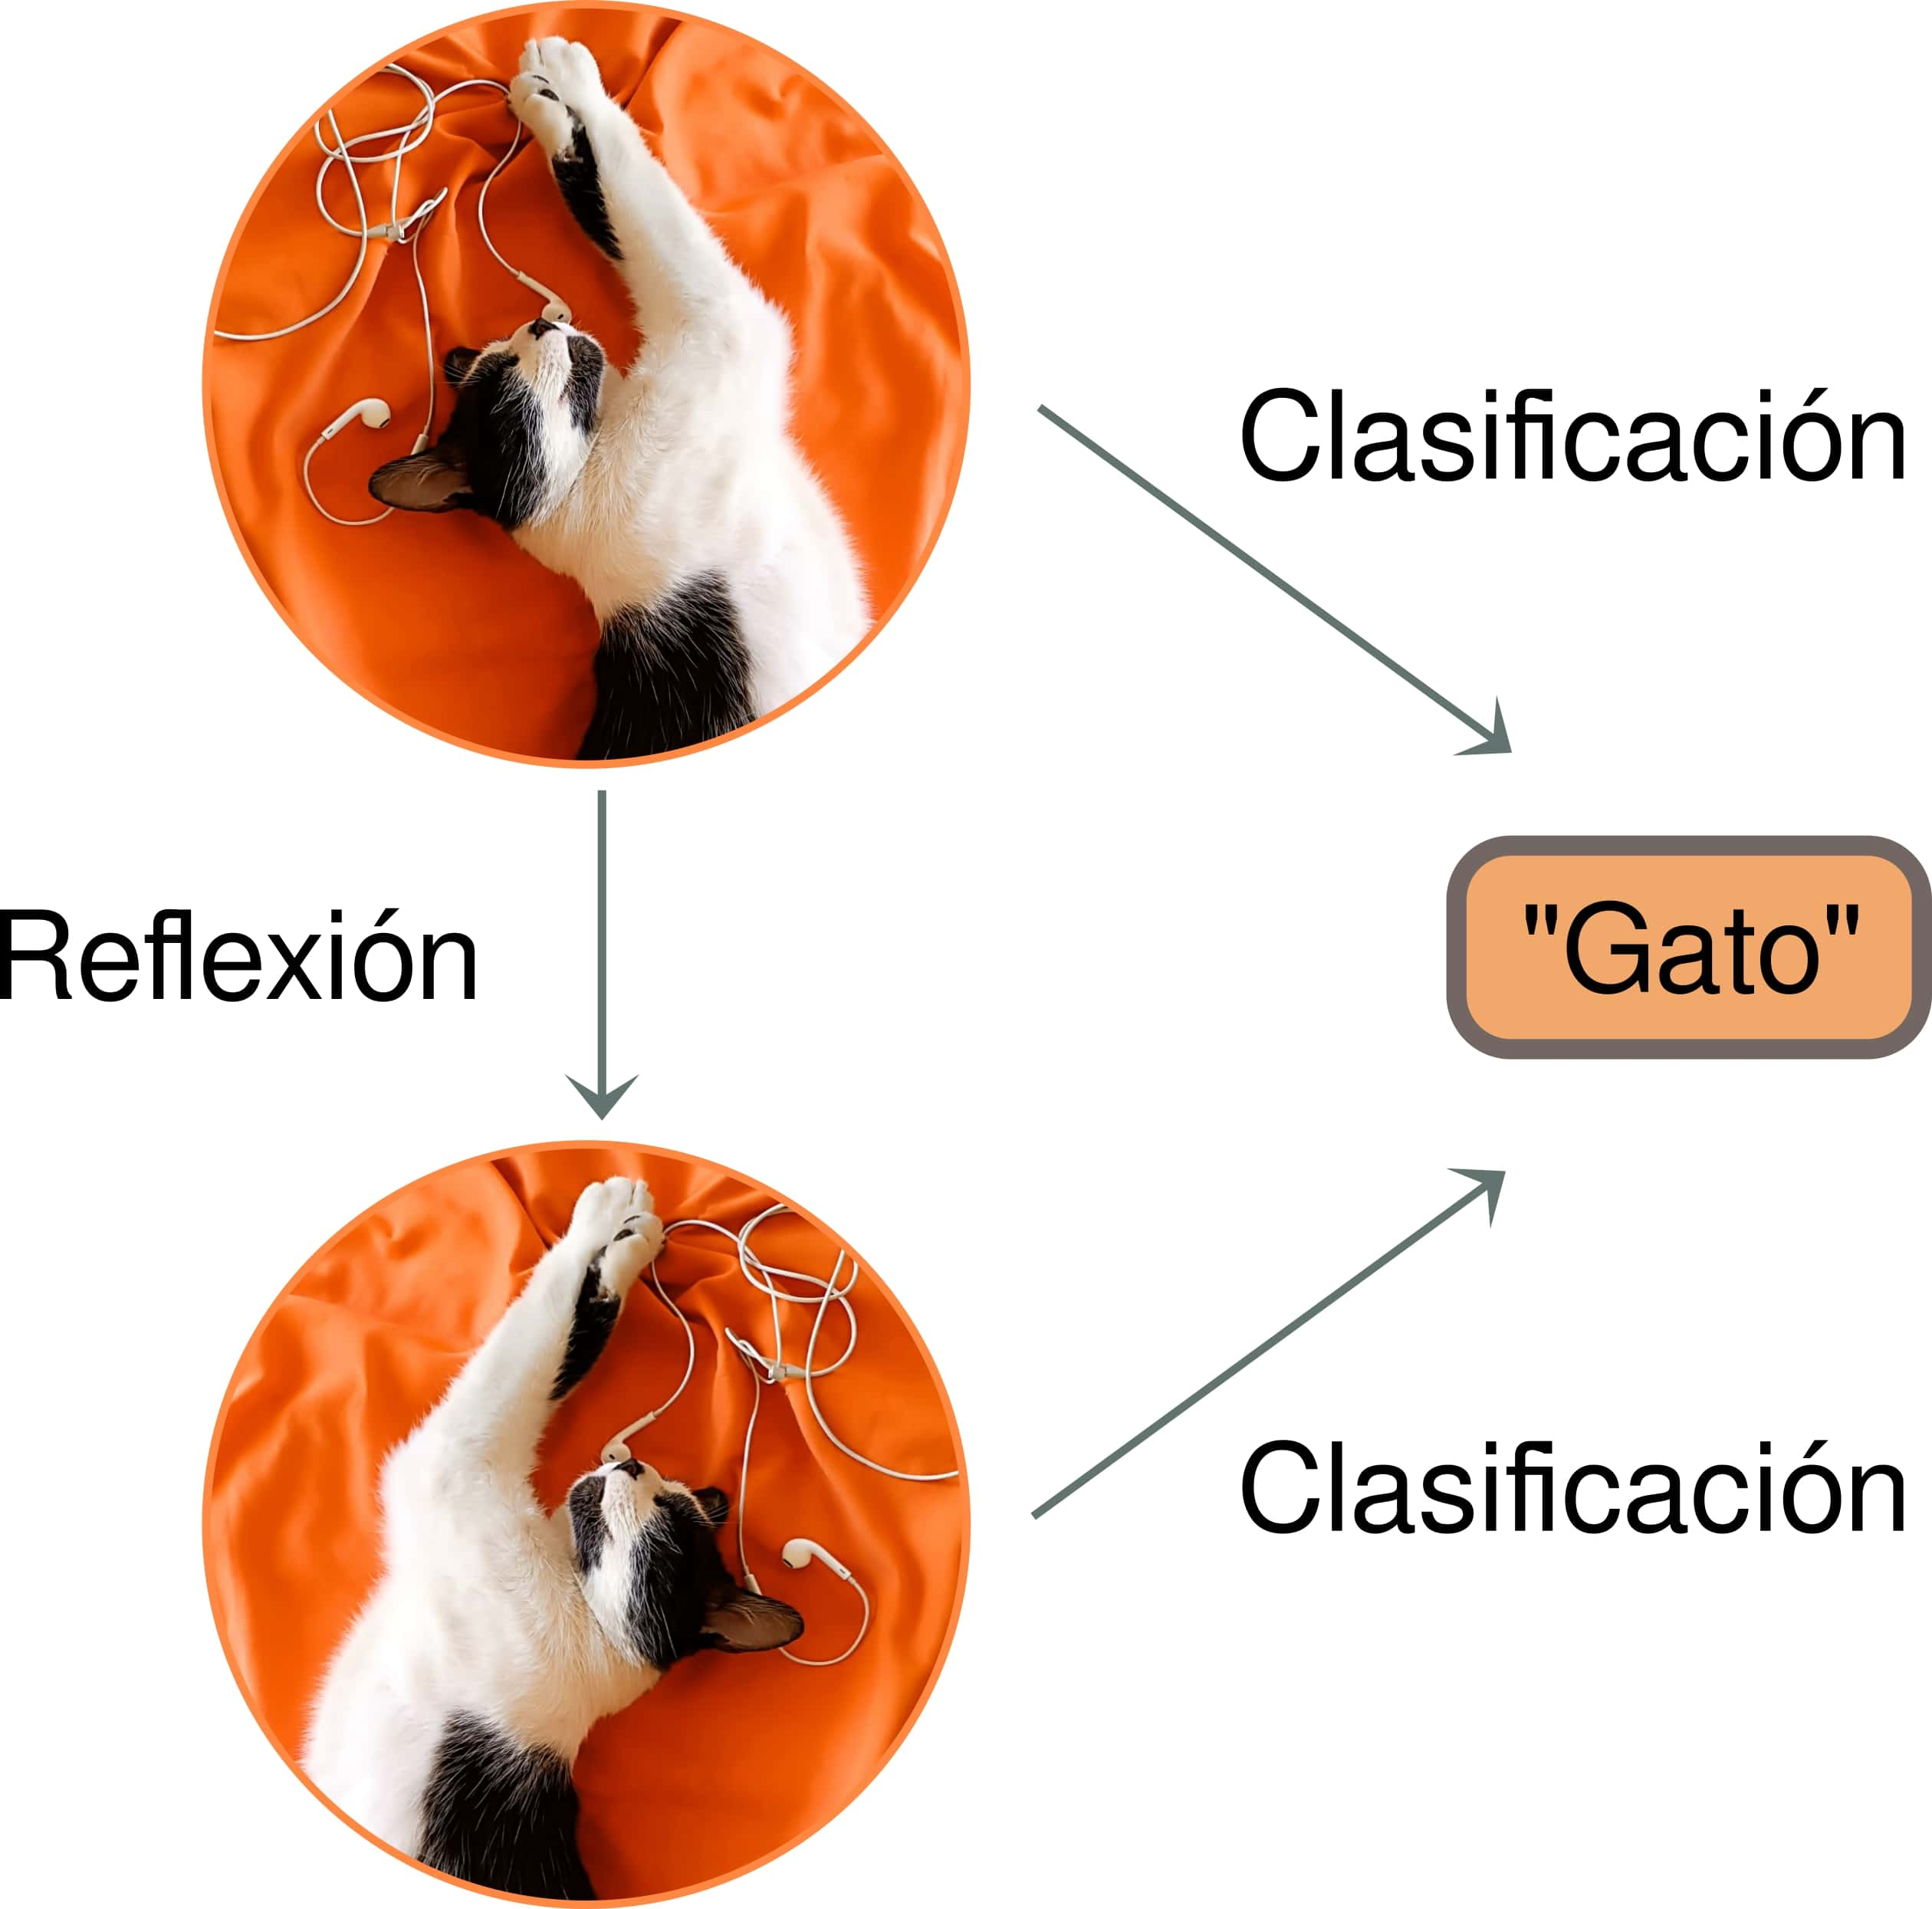
\includegraphics[width=0.35\linewidth]{fig2.jpg}}
\quad
\subcaptionbox{Equivarianza}{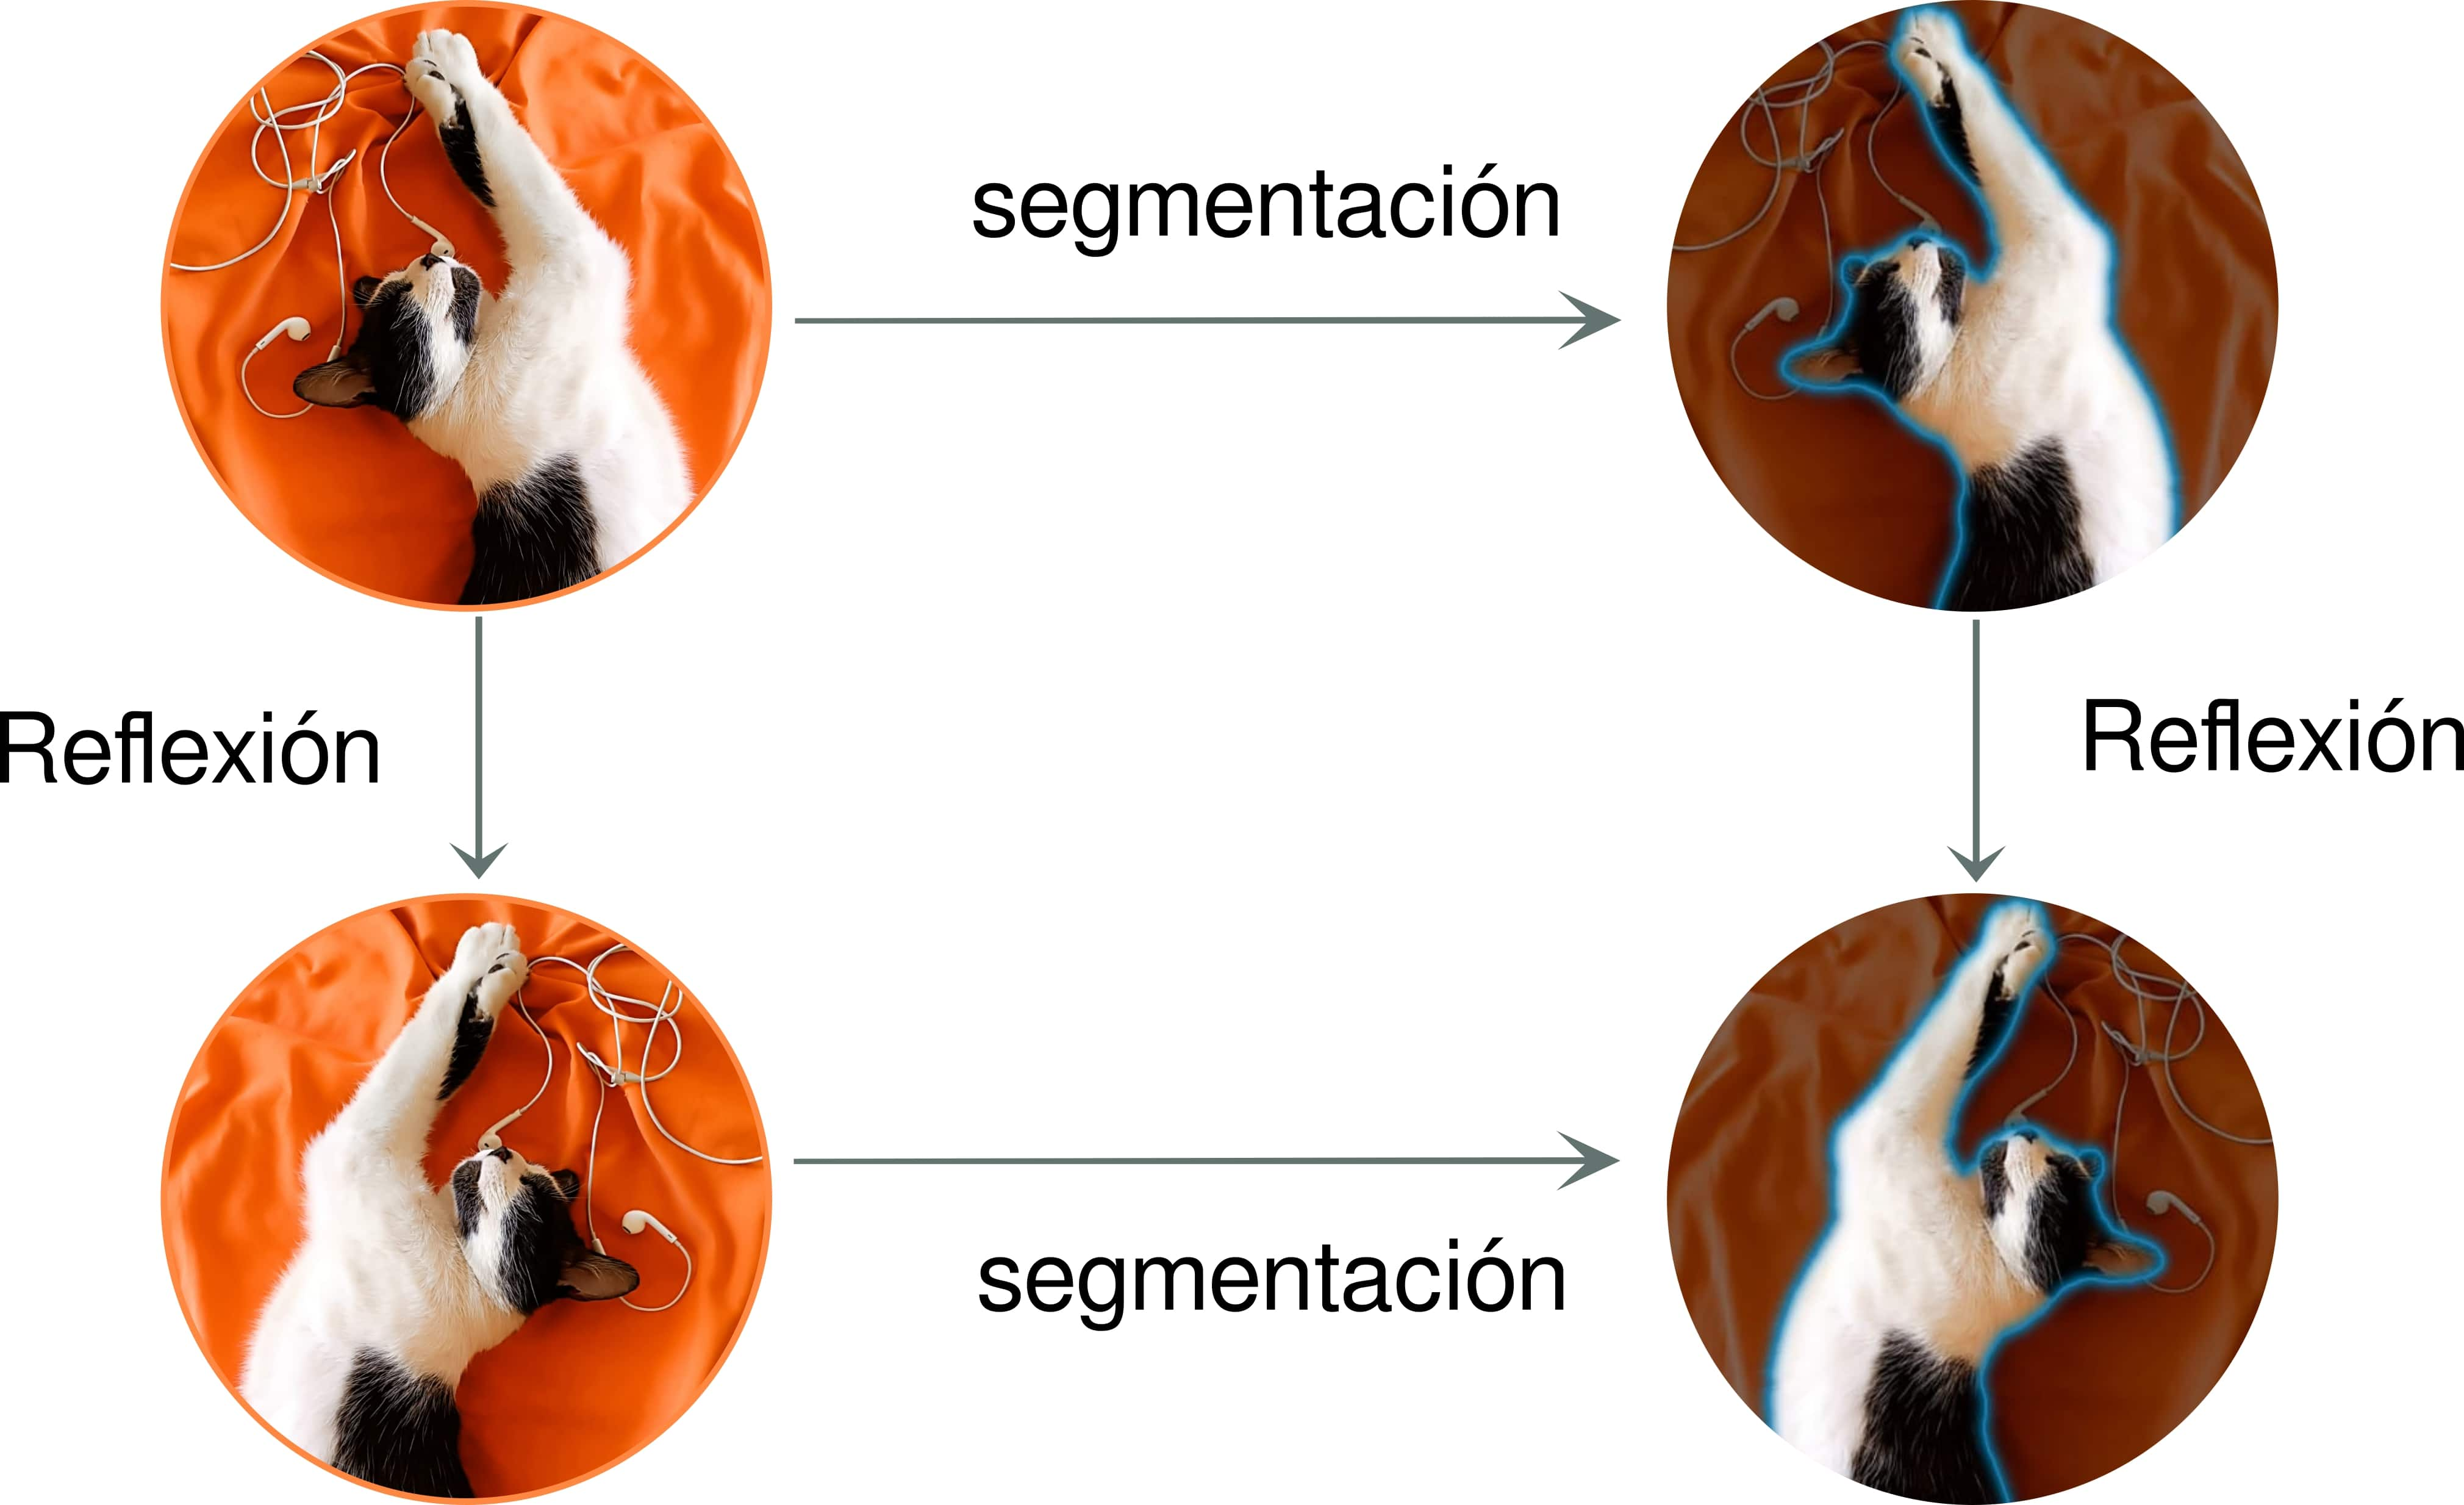
\includegraphics[width=0.55
\linewidth]{fig3.jpg}}
\caption{En \textbf{(a)} se muestra cómo la clasificación puede ser invariante.
    En \textbf{(b)} se muestra cómo la segmentación puede ser equivariante.}
\label{fig:cat_segmentation}
\end{figure}


A estas funciones caracterizadas por transformaciones que conmutan con la aplicación de la función (en este caso la red neuronal convolucional) se les llama equivariantes, en este caso, al grupo de simetría de las traslaciones \cite{lim_what_2022}. Es decir, el proceso de aplicar una transformación de simetría y luego calcular la función que produce el mismo resultado que calcular la función y posteriormente aplicar la transformación.

En el caso particular de datos que va ser usado en el presente proyecto, esto es - las imágenes histopatológicas, estas se caracterizan en que además de contar con este tipo de simetría traslacional, no presentan una orientación preferida, es decir, un conglomerado celular presenta las mismas características morfológicas sin importar si la imagen es reflejada o rotada arbitrariamente y, por lo tanto, en la práctica, un patólogo puede obtener el mismo diagnóstico sin siquiera haber notado que la imagen ha sido previamente rotada. Esta característica de las imágenes histopatológicas las hace diferente de otros tipos de imágenes que sí presentan una orientación preferida, como es el ejemplo claro de los dígitos y en particular los números: $6$ y $9$, como se aprecia en la Figura \ref{fig:69}.

\begin{figure}[h!]
    \centering
    
\includegraphics[width=0.3\textwidth]{6.jpg}
    
\includegraphics[width=0.3\textwidth]{9.jpg}
    \caption{Un ejemplo de que no todas las imágenes tienen simetría rotacional, en particular los dígitos $6 $ y $9$ se diferencian por una rotación de 180°}
    \label{fig:69}
\end{figure}
Como en el caso de las redes neuronales convolucionales usuales, aprovechar esta simetría ofrece un sesgo inductivo fuerte a los modelos de aprendizaje ya que reduce los grados de libertad que los modelos y sus parámetros pueden tener y -tal como en las redes convolucionales usuales,- permite hacer weight sharing lo que las hace menos propensas a overfitting, permitiéndoles converger más rápidamente con una menor cantidad de datos \cite{cesa_program_2021}. De hecho, uno de los métodos usado para lograr estas mismas características en una red consiste en el conocido data augmentation con transformaciones geométricas del dataset, sin embargo, el uso de estas simetrías concretamente en este contexto equivariante de imágenes histopatológicas es estrictamente más efectivo que realizar data augmentation con transformaciones geométricas \cite{elesedy_provably_2021}.
%Esta es la cita: \cite{elesedy_provably_2021}.
%tra cita \cite{franzen_general_2021}

\paragraph{Grupo}

Para poder describir una simetría en lenguaje matemático usualmente se habla de grupos. Un grupo en matemáticas hace referencia a un conjunto no vacío creado a partir de una operación que combina cualquier par de elementos que sean parte del grupo para obtener un tercer elemento que también cumplirá con las condiciones de dicho grupo.

Los grupos son usados en diversas áreas de la matemática. Especialmente, en la geometría sirven para agrupar las simetrías o diferentes transformaciones geométricas con respecto a un objeto geométrico determinado. Lo anterior quiere decir que las simetrías de un objeto geométrico forman el grupo de simetrías, mientras que cierta transformación tal como la rotación forma el grupo de rotaciones en una esfera, por ejemplo.

Para efectos prácticos un objeto geométrico puede ser una línea o una esfera, pero los grupos se pueden definir de manera más abstracta, lo que permite hablar de otros y más diversos tipos de simetrías.
De acuerdo a lo anterior, para que un grupo dado sea considerado como tal requiere que sea un conjunto que contenga al menos las siguientes reglas de combinación, también conocidas como axiomas del grupo. Para todo $a,b,c,e \in G$ un grupo, usando como notación usual la de la operación de multiplicación se tiene:
La operación es asociativa
\begin{equation}
(ab)c=a(bc)
\end{equation}
Tiene un elemento de identidad $e$.
\begin{equation}
ea=ae=a
\end{equation}
Cada elemento del conjunto tiene un elemento inverso.
\begin{equation}
a^{-1}a=aa^{-1}=e
\end{equation}

\paragraph{Grupo de Simetría}

La forma en que el concepto de grupo captura la idea de simetría es por medio del concepto de grupo de simetría. El grupo de simetría es un grupo de acciones o transformaciones que al aplicarse a un objeto matemático no modifican sus características generales, es decir, se mantiene invariante. Un ejemplo de lo anterior son las rotaciones de una esfera. Es así como los objetos que presentan simetrías pueden ser objetos geométricos, imágenes, ecuaciones en física o patrones en general. Así mismo, el elemento de un grupo puede actuar sobre un conjunto o espacio, un concepto altamente correlacionado con la simetría, pues la simetría es un tipo de invarianza en donde un objeto no cambia después de ser transformado por alguna acción particular.

Para el presente trabajo de investigación, los grupos a considerar son grupos de simetría, en particular, las simetrías que tienen las imágenes histopatológicas: traslación, rotación y reflexión, incluidas sus combinaciones. Algo que puede sonar similar al concepto de data augmentation, donde a un conjunto de datos se les aplica este mismo tipo de transformaciones geométricas para aumentar el tamaño del conjunto; pero en el caso de las redes equivalentes se desea agregar esta información de grupo de simetría directamente en la red, no solo en los datos con los que se entrena.


\paragraph{Mapas equivariantes o funciones equivariantes}

Son funciones para las cuales la entrada y la salida reciben la misma acción del grupo (la acción del grupo conmuta con la aplicación de la función). Esto quiere decir, que es posible `factorizar' la acción de un grupo de la función. Formalmente, la equivarianza se puede describir como:

Sea $g \in G$ elemento de un grupo que actúa en $X,Y$, el dominio y codominio de una función $f$. Se dice que esta función $f \colon  X \to Y $ es equivariante a la acción del grupo $G$, si para todo $g$:
\begin{equation}
f(g \cdot x)=g \cdot f(x)
\end{equation}
Esta propiedad también se puede ver como un diagrama conmutativo:
\begin{center}
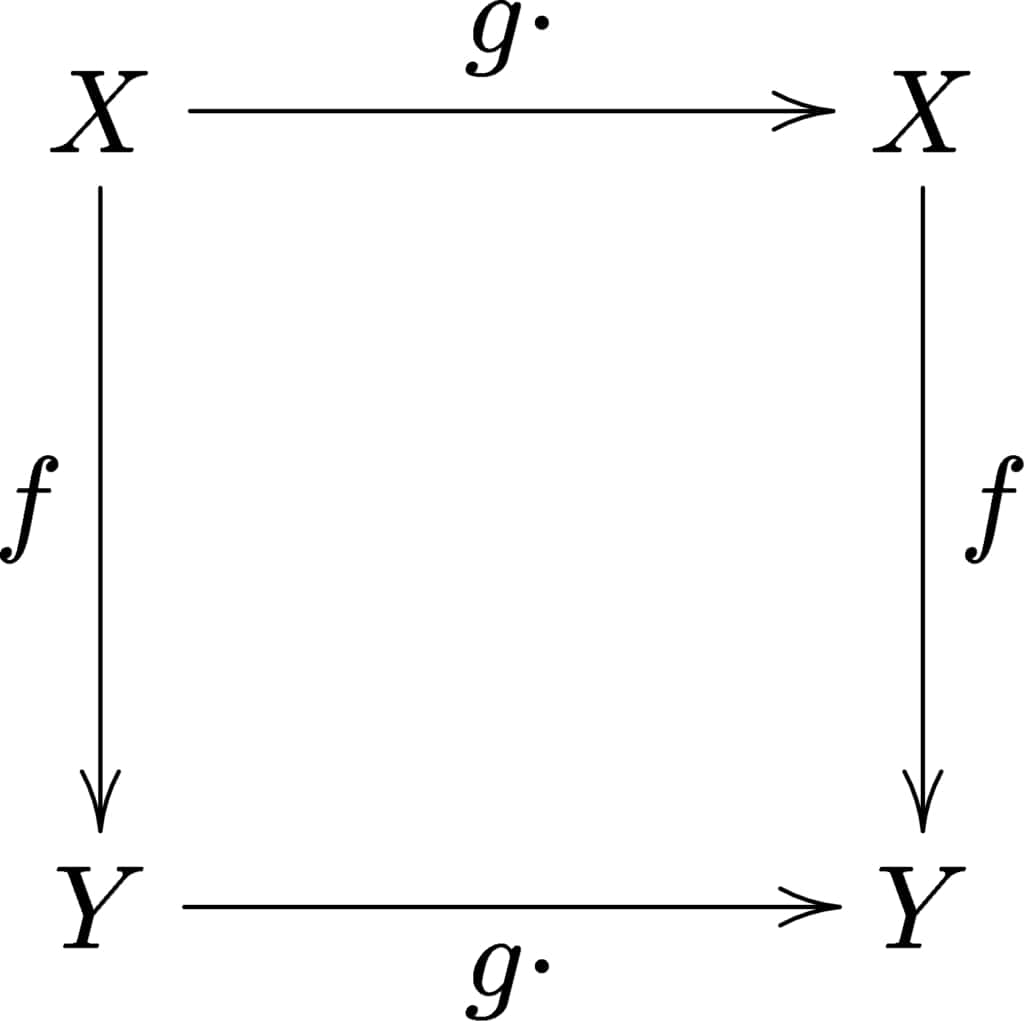
\includegraphics[scale=0.1]{equivariance_diagram.jpg}
\end{center}
\paragraph{Convolución en grupos}
La convolución en grupos es una operación similar a la convolución tradicional discutida anteriormente, solo que ahora son funciones definidas en un grupo $f,g \rightarrow G$. Estas convoluciones presentan abundantes características similares a las tradicionales, algo semejante a mezclar dos funciones, solo que ahora definidas en un grupo (de simetría, para este trabajo), lo que permite aprovechar las simetrías que tiene la señal, pues además de las características usuales de la convolución tradicional, esta convolución en grupos permite usar la estructura que dan los grupos, permitiendo equivarianza, esto es, la aplicación del grupo a la convolución conmuta con la aplicación a la función (derecha o izquierda de la convolución, pues de manera general la multiplicación en grupos no es conmutativa) esto se puede ver en la Figura \ref{fig:conv_equivariant}. Sumado a esto, en \cite{kondor_generalization_2018} se demostró que la convolución en grupos no solo es una condición suficiente para mapas o funciones equivariantes, sino una condición necesaria. Por lo que, de manera general, las redes neuronales equivariantes hacen uso de convoluciones en grupos.

\begin{figure}[h!]
    \centering
    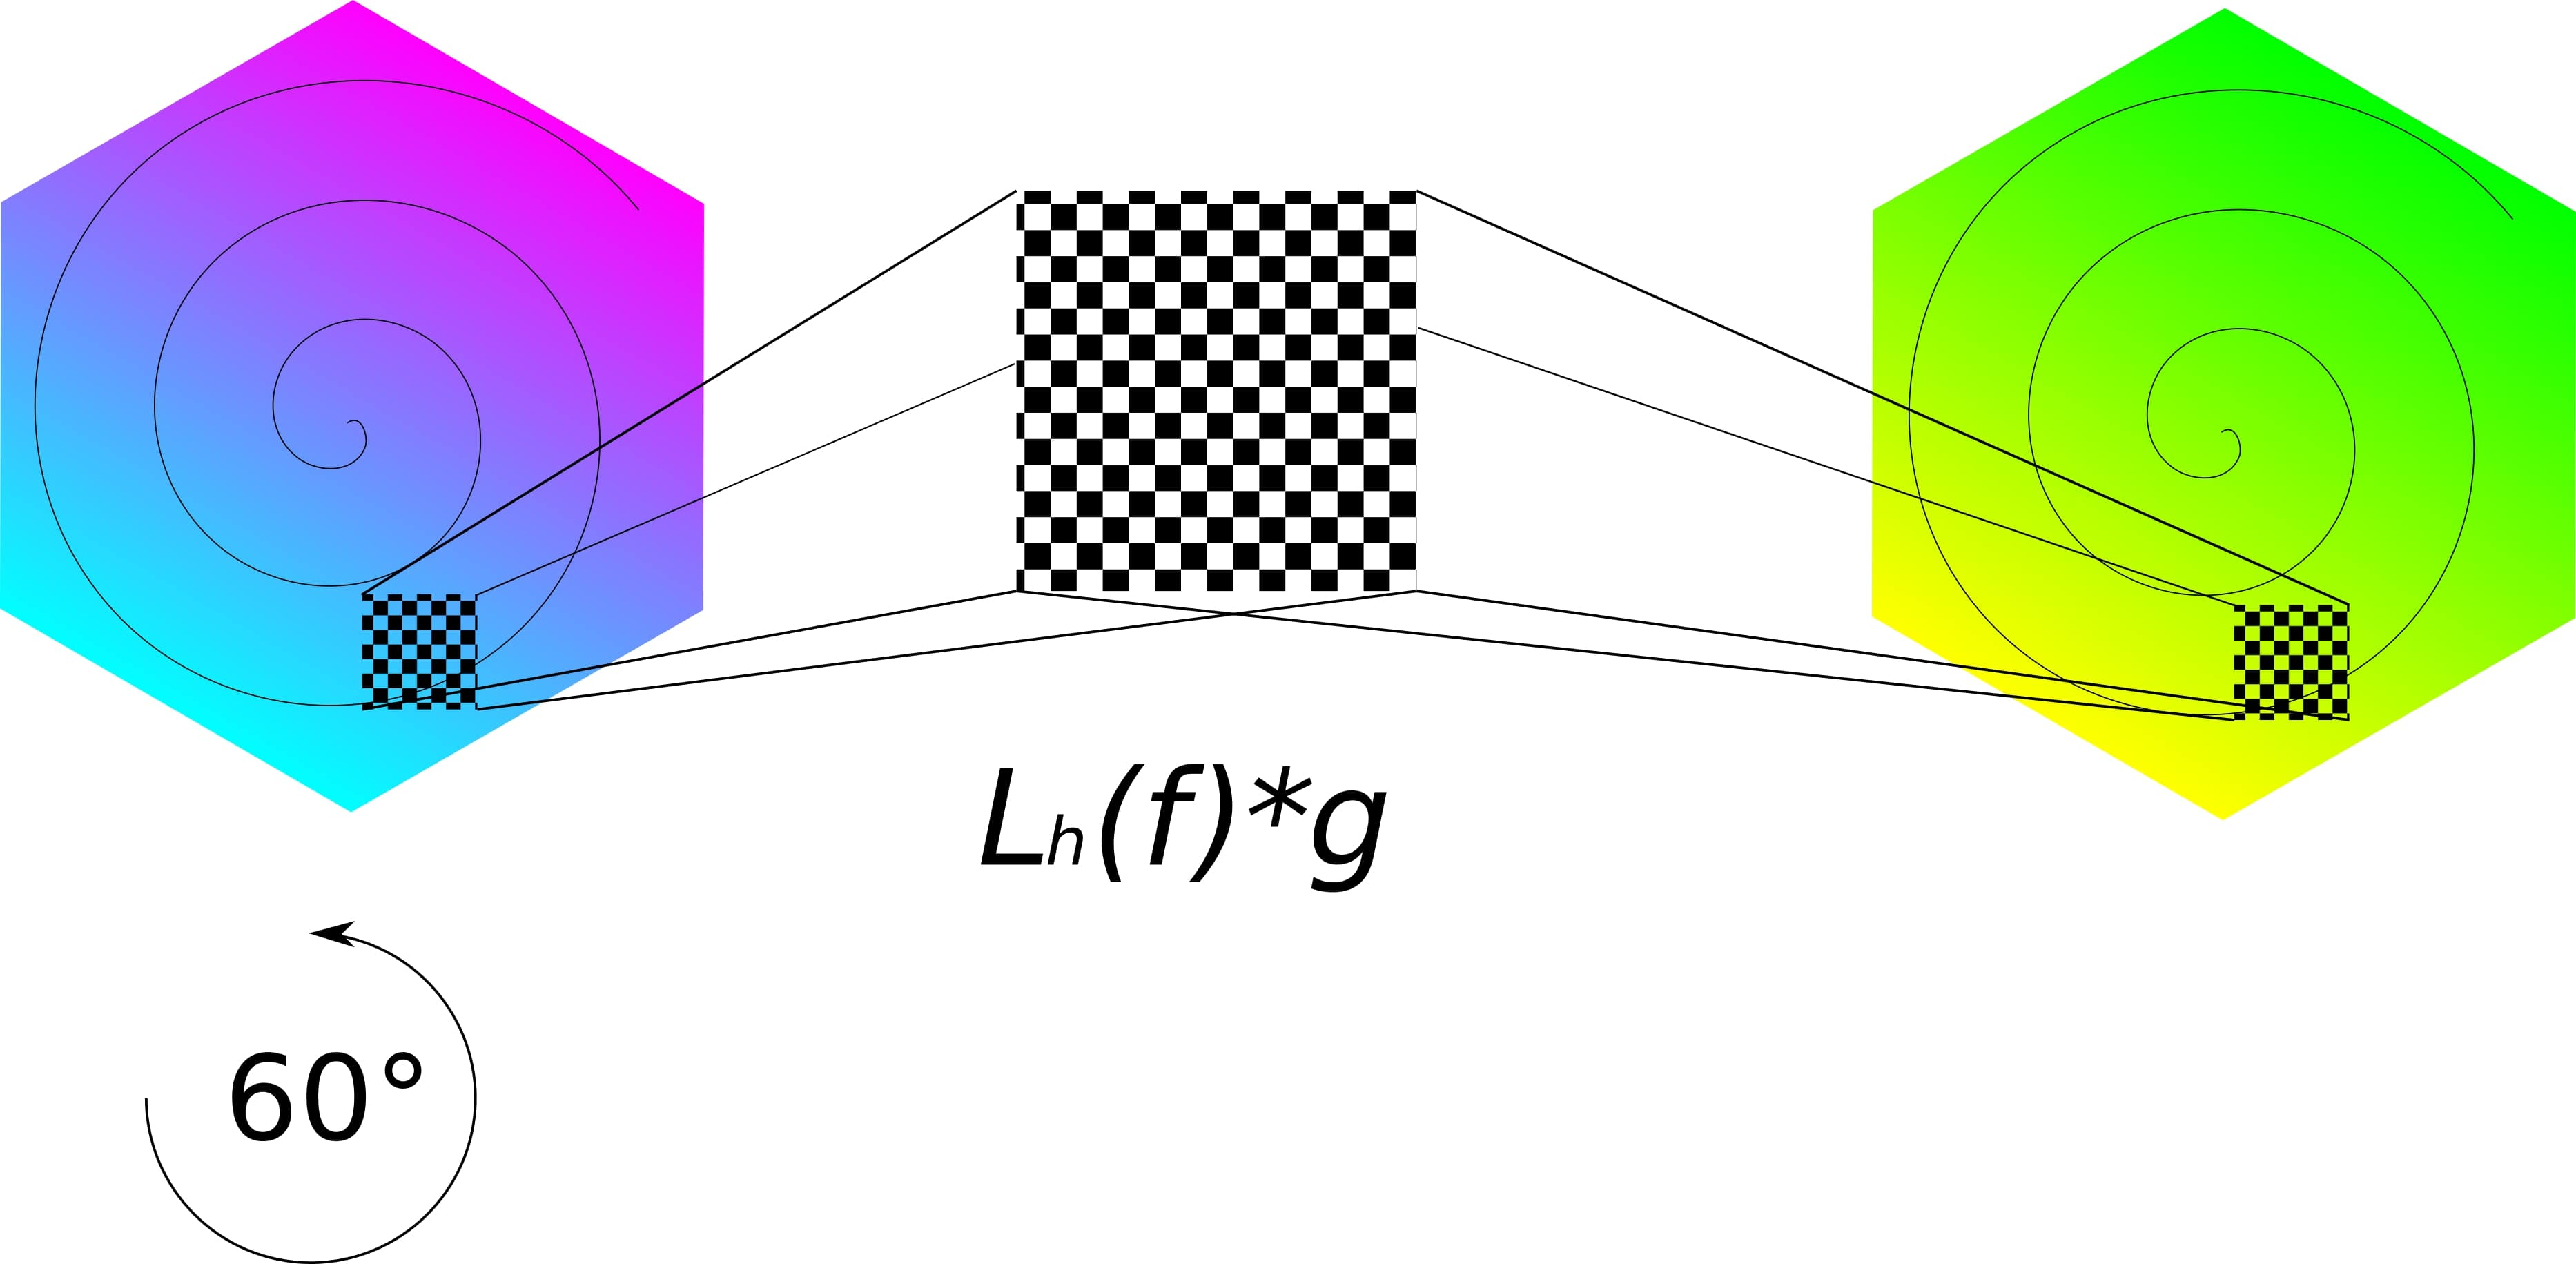
\includegraphics[width=0.45\textwidth]{aplicacion_en_f.jpg}
    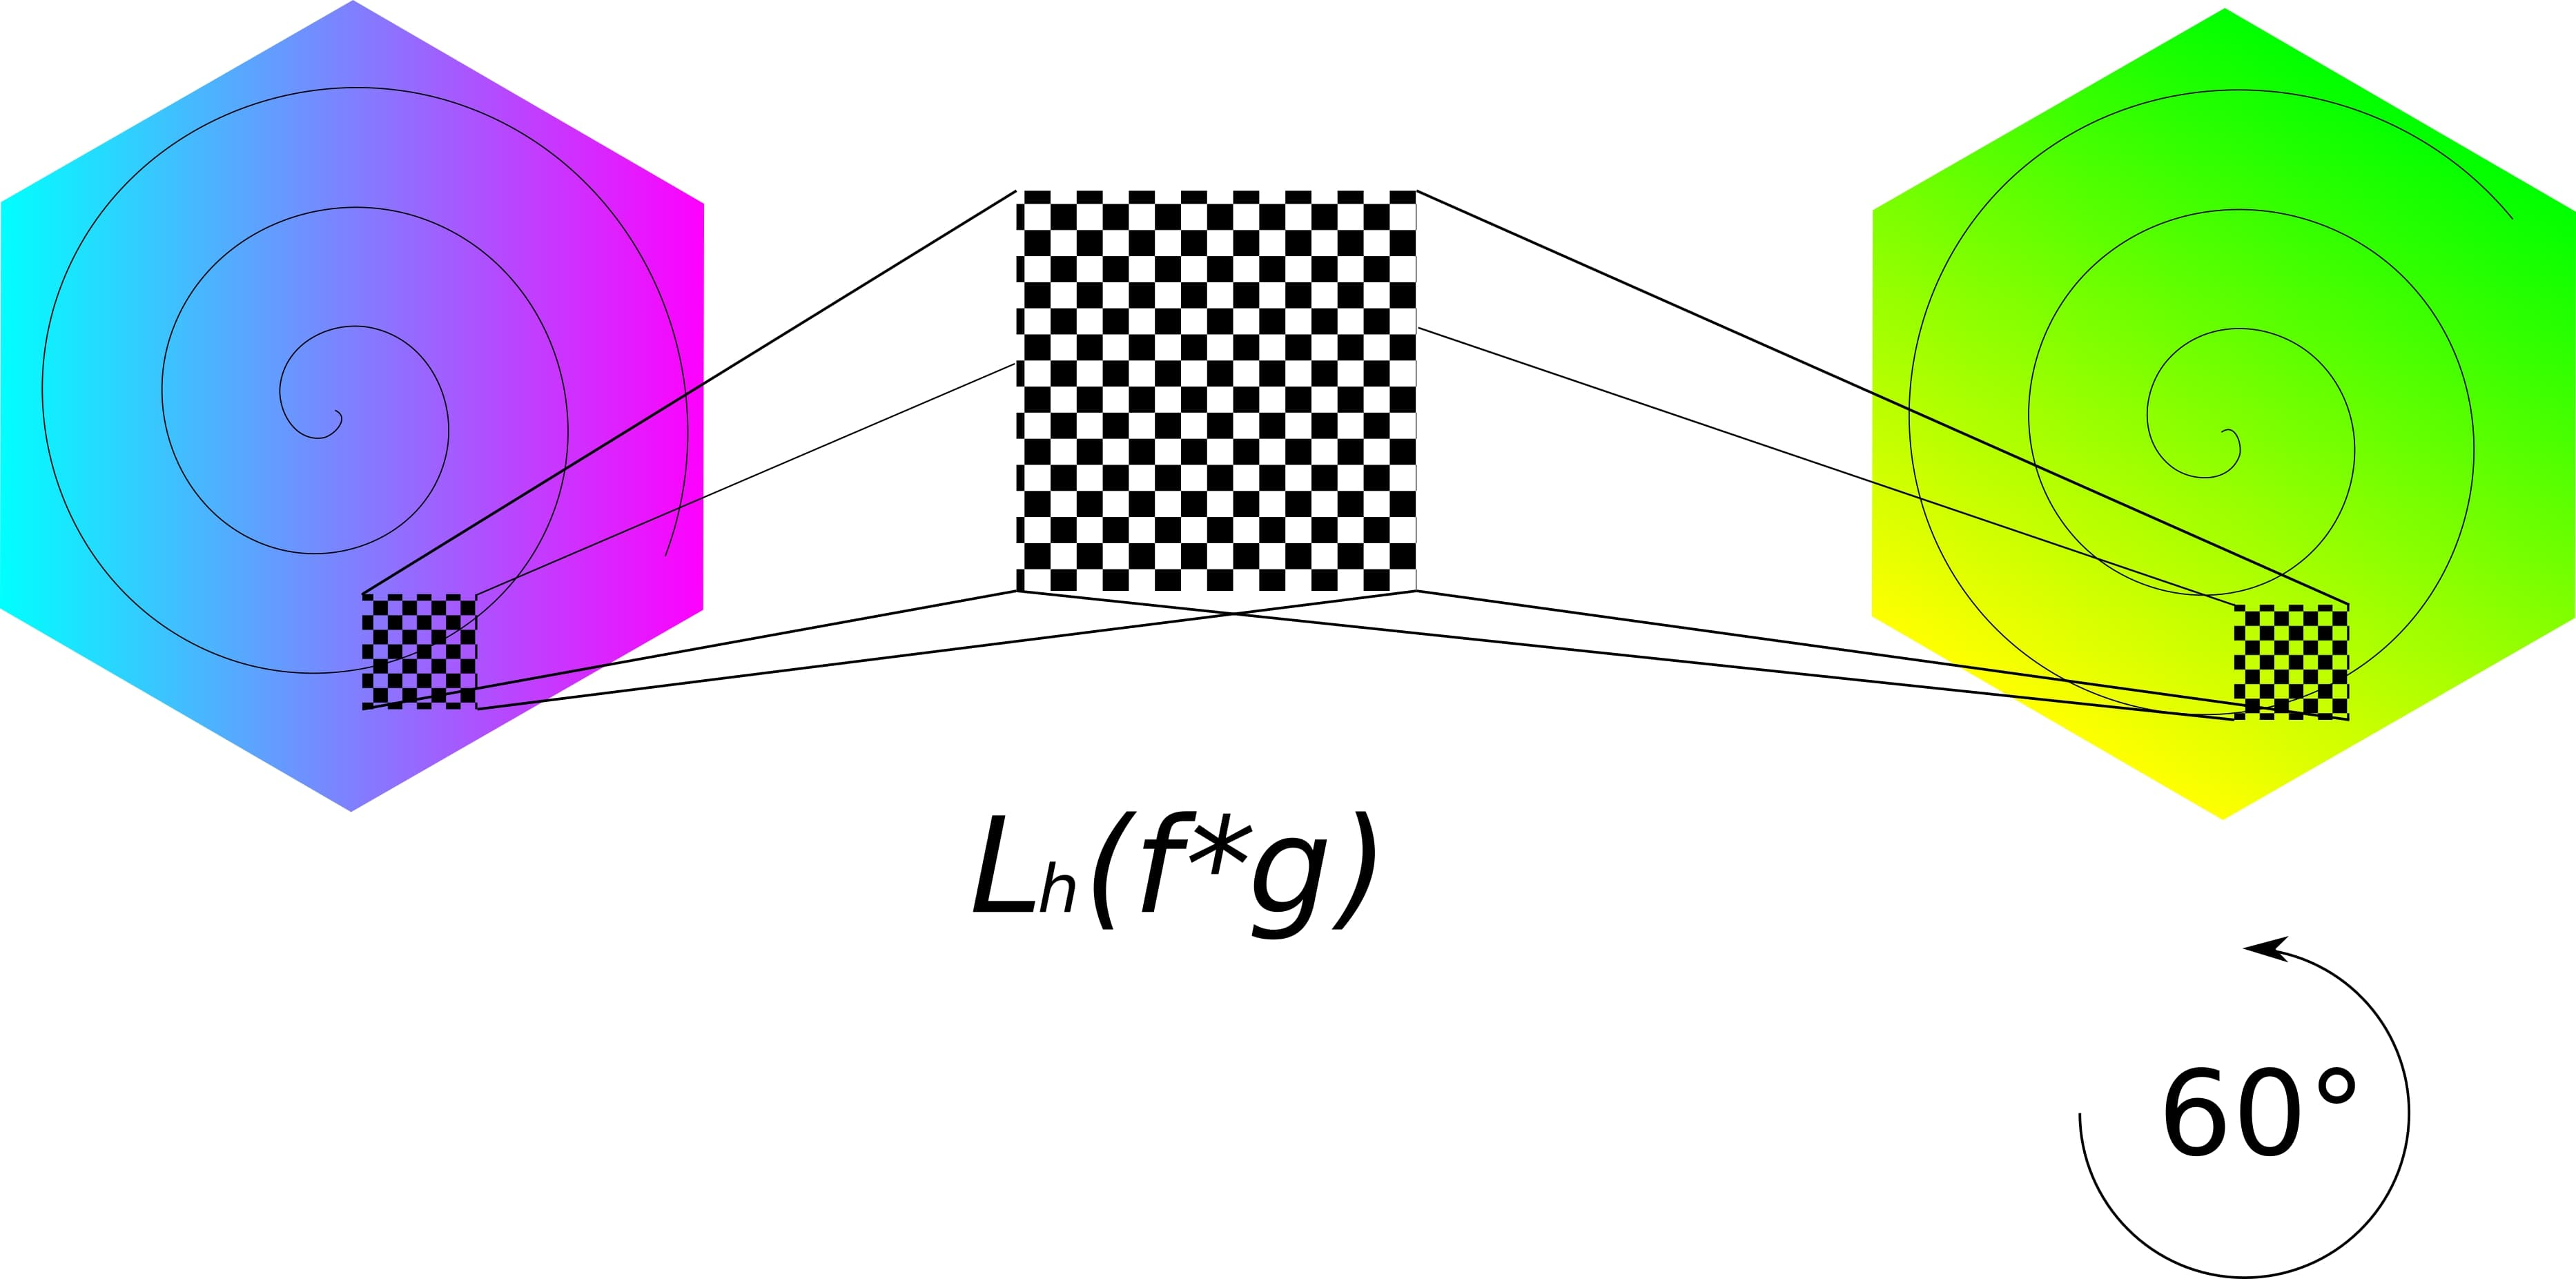
\includegraphics[width=0.45\textwidth]{aplicacion_en_fg.jpg}
    \caption{Ejemplo de la equivarianza de la convolución en grupo de simetría a las rotaciones de $60^{\circ}$. El filtro se desliza sobre el hexágono y va transformando los colores: no importa si primero se rota el hexágono de entrada (imagen izquierda), o si se rota el resultado de la convolución (imagen derecha). Como resultado, el gradiente de color en el hexágono de salida es el mismo.}
    \label{fig:conv_equivariant}
\end{figure}

La convolución en grupos, entonces, se define similarmente a la tradicional, de la siguiente manera:

\begin{equation}
(f * g)(x) = \int_{G} f(y)g\ (y^{-1} x)\  d\lambda(y)
\end{equation}

Donde $d\lambda$ es una medida (measure en inglés) -por la izquierda o por la derecha solamente, pues no se puede asumir conmutatividad de la operación del grupo- de Haar y $x, y$ pertenecen a un grupo $G$. Se puede notar el alto grado de similitud con la convolución tradicional y, de hecho, si tomamos $(\mathbb{R},+)$ como un grupo $G$ (números reales con la operación suma), se obtiene la convolución tradicional completa.



Este tipo de convolución tiene la propiedad importante de que la acción del grupo (por la izquierda) $L_{h}$ a la función $f$ conmuta con la convolución, es decir:

\begin{equation}
L_{h}(f * g) = (L_{h}f) * g
\end{equation}


\begin{figure}[h!]
    \centering
    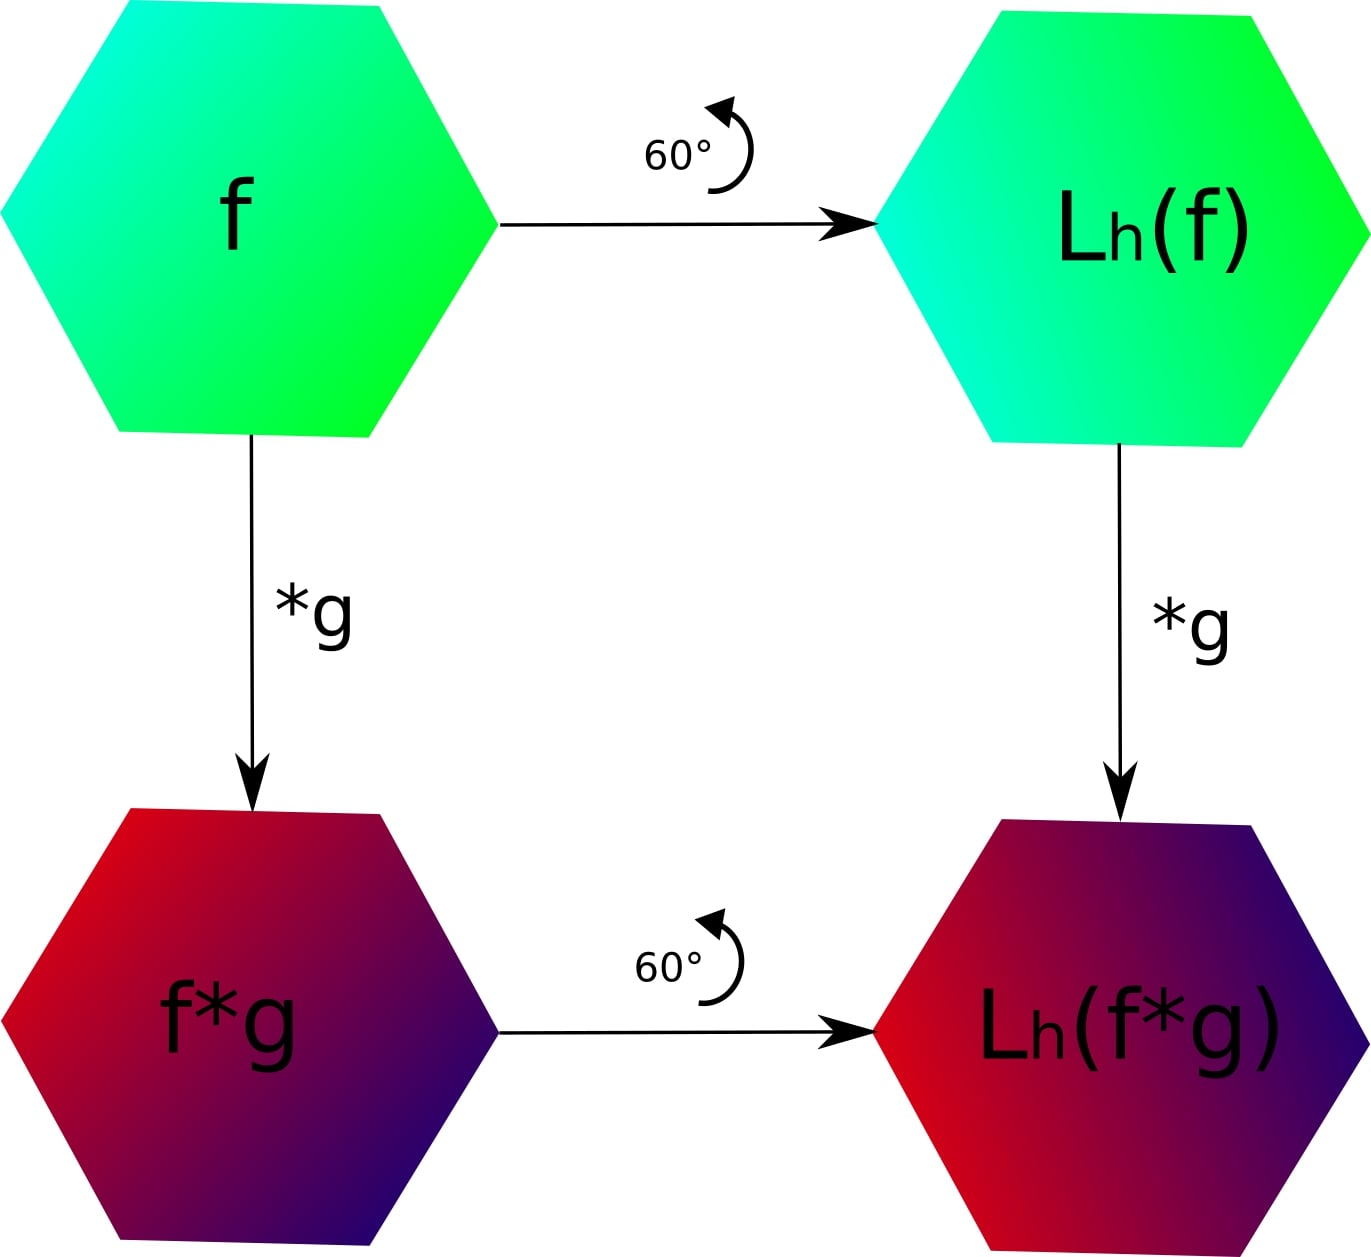
\includegraphics[width=0.5\textwidth]{hexagono.jpg}
    \caption{Los hexágonos tienen simetrías rotacionales de $60^{\circ}$, por lo que el grupo de rotaciones de $60^{\circ}$ actúa como un grupo de simetría que actúa sobre los hexágonos. También se puede observar como una función definida en un hexágono (en este caso representada por el gradiente de color) cumple con el diagrama conmutativo que requiere la equivarianza: si se fija una función $g$ (que al igual que $f$ se representa como un gradiente de color) con la que se realiza la convolución, se puede observar cómo es equivariante primero rotar el hexágono con la acción del elemento del grupo $L_{h}$, una rotación de $60^{\circ}$ o primero realizar la convolución $f*g$ y luego aplicar la acción del grupo.}
    \label{fig:convdiagram}
\end{figure}

Esta es justamente la propiedad de equivarianza que se busca y que presenta la convolución en grupos. Esto se puede ver fácilmente en la figura \ref{fig:convdiagram}.



\section{Trabajos Previos en Redes neuronales Equivariantes}


En la presente sección se presentan los avances más relevantes dentro del estado del arte actual referente a la teoría, implementación y uso de redes neuronales equivariantes en general y aplicados en imágenes histopatológicas en particular.

Una de las primeras descripciones generales del uso de convoluciones en grupos para obtener equivarianza se puede ver en ``Group Equivariant Convolutional Network" de Cohen \& Welling en 2016 \cite{cohen_group_2016},  donde realizaron una descripción teórico-matemática detallada de qué es una convolución en un grupo y se explican algunos detalles para su discretización en código, presentando un nuevo tipo de capa que usa convoluciones en grupos discretos para obtener equivarianza. También muestran resultados del estado del arte en benchmarks comunes como lo son el dataset MNIST rotado y CIFAR10 (2.28\%error y 4.19\% y. 6.46\% en CIFAR10 aumentado y sin aumentar).

Además, Cohen \& Welling  también son los encargados de describir la teoría de los filtros orientables para el uso de las redes neuronales convolucionales bajo la teoría de la equivarianza en grupos en ``Steerable CNNs"\cite{cohen_steerable_2016}. Una teoría que será usada para la implementación de la CNN en las imágenes histopatológicas en la presente tesis. En este trabajo, de nuevo obtuvieron resultados del estado del arte incluso bajo regímenes de entrenamiento con pocos datos, comparando con ResNet y redes que usan transfer learning. Para este trabajo Cohen \& Welling se basaron en teoria tradicional de filtros orientables (steerable filters). En particular, Freeman \& Adelson (1991) son los investigadores que inicialmente introducen la teoría clásica de los filtros orientables para visión por computador y detalles de su implementación en código en su trabajo inaugural: ``The design and use of steerable filters"\cite{freeman_design_1991}.

Por otra parte, avances importantes en el campo relevantes para este trabajo de tesis, como los llevados a cabo por Elesedy \& Zaidi en 2021 en su trabajo ``Provably Strict Generalisation Benefit for Equivariant Models" \cite{elesedy_provably_2021} donde se encargan de demostrar formalmente que las redes neuronales equivariantes son estrictamente mejores y más eficientes en el entrenamiento y generalización con datos que son equivariantes a la acción de un grupo, comparado con otros métodos como data augmentation. En particular, para imágenes, que presentan equivarianza traslacional, se obtienen las mismas redes convolucionales usuales.

De manera más reciente, Cesa et al. \cite{cesa_program_2021} muestran el proceso matemático para la construcción de redes convolucionales equivariantes para el grupo euclidiano y todos sus subgrupos. Además implementan en código este tipo de redes de manera general en una librería de Pytorch. Por otra parte, generalizan el teorema de Wigner-Eckart para todos los grupos compactos para poder encontrar representaciones irreducibles de estos grupos, que es un paso fundamental en la implementación de este tipo de redes.

Cabe destacar que durante ese mismo 2021, Weiler, Maurice, et al. \cite{weiler_coordinate_2021} presentaron la que sería la formulación teórica más general de una red equivariante, requiriendo solamente equivarianza a los gauges de variedades riemannianas e implementan una red neuronal convolucional en una banda de Möbius en ``Coordinate Independent Convolutional Networks--Isometry and Gauge Equivariant Convolutions on Riemannian Manifolds".


Así mismo, Bekkers, et al. \cite{bekkers_roto-translation_2018}, muestran el uso de redes equivariantes para imágenes médicas (incluido imágenes histopatológicas) en el trabajo denominado ``Roto-Translation Covariant Convolutional Networks for Medical Image Analysis". En este artículo se implementa una red neuronal convolucional equivariante al grupo euclidiano (el grupo de traslaciones, rotaciones y reflexiones), obteniendo resultados comparables con el estado del arte sin necesidad de hacer uso de la técnica de aumento de datos. Entre las imágenes médicas con las que experimentan con este modelo se encuentran datasets de imágenes histopatológicas para detección de mitosis, segmentación de vasos sanguíneos en retícula y segmentación de células de imágenes de microscopio de electrones. En el caso de este trabajo, se usan rotaciones discretas y empíricamente se observa que entre más fino es el sampling de las rotaciones, por ejemplo tomando rotaciones de 30° en vez de 90°, se mejoran los resultados y se disminuye la varianza.
\\
Por último, es menester citar dos trabajos que son parte de los antecedentes del presente proyecto: En primer lugar, de 2018 ``Rotation Equivariant CNNs for Digital Pathology" de Veeling, et al. \cite{veeling_rotation_2018} muestran que las imágenes histopatológicas son invariantes a la reflexión y a la rotación e implementan una red neuronal convolucional equivariante a la rotación de 90°, mostrando que utilizar redes equivariantes para imágenes histopatológicas mejora sustancialmente el rendimiento incluso con menos parámetros. En segundo lugar, de 2020 ``A Dynamic Group Equivariant Convolutional Networks for Medical Image Analysis" de Li, Cao, \& Cao. \cite{li_dynamic_2020} donde desarrollan convoluciones dinámicas en el framework de las redes equivariantes. Estos autores generalizan las convoluciones dinámicas, que es una forma de \textit{atención}, sobre los filtros de redes convolucionales. En este caso, también utilizan imágenes histopatológicas de cáncer de mama para validar un modelo de red convolucional dinámica y equivariante y obtienen resultados del estado del arte.
Como se puede ver, existen métodos equivariantes para clasificación supervisada. También existen una importante cantidad de métodos no supervisados que no son equivariantes. Explorar esta idea en enfoques de aprendizaje no supervisado, como se plantea en este proyecto, puede resultar interesante, pues el sesgo inductivo asociado a la equivarianza podría llevar a representaciones más efectivas de las imágenes histopatológicas.



%% SOBRE LA INVESTIGACIÓN %%%%%%%%%%%%%%%%%%%%%%%%%%%%%%%%%%%%%%%%%%%%%%%%%%%%
\newpage
\chapter{Planteamiento del problema y justificación}

La histología es una de las ramas fundamentales de la medicina ya que esta rama de la ciencia esta encargada en el estudio de la anatomía de los seres humanos desde una perspectiva microscópica. Es así como la histología ha posibilitado avances cruciales para el diagnóstico de enfermedades a través de la identificación de síntomas a nivel microscópico en el campo de la patología médica. Esto se debe a que la capacidad de examinar los tejidos a nivel celular ha ayudado a comprender la naturaleza y el desarrollo de las enfermedades. En el caso específico de patologías asociadas al cáncer, la histología ha desempeñado un papel vital identificando alteraciones morfológicas y celulares asociadas con los diferentes tipos de tumores.

En la actualidad, la digitalización de imágenes histopatológicas ha permitido el desarrollo de la patología digital. La adquisición digital de láminas histológicas completas permite su almacenamiento, análisis y distribución de manera eficiente. Esta transformación tecnológica ha superado las limitaciones tradicionales de la patología facilitando el acceso remoto a las imágenes y promoviendo la colaboración entre profesionales de la salud en diferentes ubicaciones geográficas. Ambos aspectos prometen un avance significativo en el proceso de diagnosis de cáncer.

Entre las herramientas computacionales asociadas a la patología digital, los sistemas de apoyo al diagnóstico prometen mejorar la precisión y la eficiencia en la toma de decisiones médicas. La posibilidad de aplicar herramientas automáticas de análisis ha impulsado la investigación y el desarrollo de enfoques más avanzados para la detección y clasificación de enfermedades usando información microscópica, incluyendo el cáncer. Además, este tipo de herramientas ayudarían a reducir la alta variabilidad inter e intra observador en el diagnóstico de este tipo de imágenes.

El análisis automático de imágenes histopatológicas representa un avance en el futuro en la medicina diagnóstica. Sin embargo, los alcances de la patología digital en la actualidad está limitada por la cantidad reducida de datos anotados por expertos. Esto se debe a que recolectar imágenes histopatológicas y realizar una anotación manual implica el análisis detallado de patólogos expertos - un proceso inherentemente largo y altamente costoso.
%Por otra parte, a diferencia de otras aplicaciones comerciales, debido a las particularidades del ámbito médico, más que la eficiencia y rapidez en la inferencia de datos, es el entrenamiento y la precisión y exactitud lo que importa, dicho de otra manera, lo esencial es extraer la mayor cantidad de información con los pocos datos anotados que existan, a la vez que el modelo tenga la mayor capacidad de generalización a partir de estas limitaciones anteriormente descritas.

Para realizar el análisis automático de imágenes se han utilizado diferentes tipos algoritmos entre los que han destacado las redes neuronales profundas. Estas redes, en vez de realizar cálculos complejos y computacionalmente exigentes, permiten realizar operaciones simples pero concatenadas de forma profunda y que pueden ser ejecutadas en paralelo, disminuyendo así el tiempo de entrenamiento y de ajuste de parámetros. A cambio, necesitan gran cantidad de datos para tener una precisión adecuada en las predicciones. En general, las redes neuronales no pretenden fijar un proceso de extracción de características, sino aprender una representación adecuada que permita realizar un análisis automático.

Entre las redes neuronales para el procesamiento de imágenes, se destaca el uso de redes neuronales convolucionales que han sido revolucionarias en la medida en que son más eficientes en la cantidad de parámetros a aprender, pues aprovechan la característica de que muchos datos, en particular las imágenes, tienen información que es altamente local (por ejemplo los píxeles en una imagen tienen relación con otros píxeles adyacentes pero no con los píxeles más apartados), esto hace que requieran menos datos comparado con las redes neuronales tradicionales. Si bien el rendimiento es considerablemente mejor usando la información geométrica de estos datos, muchas observaciones son necesarias y, lamentablemente, no se aprovechan todas las simetrías que imágenes en un campo específico puedan ofrecer. Por esa razón se suele utilizar el proceso de “data augmentation”, que implica generar nuevas imágenes a partir del dataset al que se tiene acceso aplicando diversas transformaciones geométricas a las imágenes originales.

Aplicar data augmentation es ineficiente porque aumenta la cantidad de tiempo para realizar el entrenamiento, dado que, se requiere un trabajo adicional en la preparación de dataset o el preprocesamiento. Además, este procedimiento consume mayor cantidad de recursos computacionales.

Por tal motivo, en el presente trabajo de tesis se propone el uso de redes neuronales equivariantes como un método para mejorar la aplicación de las redes neuronales convolucionales a las imágenes histopatológicas. Estas imágenes tienen más simetrías que las imágenes naturales pues no tienen una orientación natural, esto es, presentan simetrías rotacionales y de reflexión, además de la traslacional. En este sentido, las redes neuronales equivariantes pueden usar de mejor manera diferentes simetrías. Esto permitiría extraer más información sin necesidad de aumentar los datos como sucede en los modelos tradicionales de aprendizaje automático.
También se propone un enfoque semi-supervisado, pues si bien hay datasets anotados por expertos, hay una cantidad enorme de imágenes no anotadas que se pueden explotar para mejorar el rendimiento de los modelos.

Esto nos lleva a formular la siguiente pregunta de investigación:

¿Puede un modelo semi-supervisado de redes neuronales convolucionales equivariantes obtener representaciones a través de un entrenamiento efectivo en comparación con modelos tradicionales (sin propiedad de equivarianza a la rotación, traslación y reflexión) entrenados en un régimen completamente supervisado para tareas de segmentación y clasificación de imágenes histopatológicas?


\newpage
\chapter{Objetivos}
\section{Objetivo General}

Desarrollar un modelo semi-supervisado de redes neuronales convolucionales equivariantes para la segmentación y clasificación de imágenes histopatológicas.


\section{Objetivos Específicos}

\begin{itemize}
    \item Seleccionar un conjunto de datos de imágenes histopatológicas anotadas que hayan sido recopiladas para la clasificación y segmentación de estructuras microscópicas.

    \item Formular e implementar un modelo semi-supervisado basado en una arquitectura de red neuronal convolucional equivariante para la segmentación y clasificación de imágenes histopatológicas.

    \item Evaluar el desempeño del modelo de redes neuronales convolucionales equivariantes sobre un conjunto de validación de imágenes histopatológicas a través de métricas para la clasificación y segmentación de imágenes.


\end{itemize}


%% METODOLOGÍA Y CRONOGRAMA %%%%%%%%%%%%%%%%%%%%%%%%%%%%%%%%%%%%%%%%%%%%%%%%%%
\newpage
\chapter{Metodología}

Para el desarrollo del presente trabajo de investigación se propone una metodología en cuatro etapas.

De cada etapa se desglosa un grupo de actividades y se evidencia el cumplimiento por medio del informe final.

% desarrollo de un informe técnico con los resultados

\section{Etapa 1. Selección de imágenes histopatológicas anotadas que hayan sido recopiladas para la clasificación y segmentación de estructuras microscópicas}

En la primera etapa se realizará una minuciosa revisión de diferentes datasets de imágenes histopatológicas para seleccionar los que permitan entrenar el modelo semi-supervisado. En este caso, se priorizarán datasets que estén completos y anotados para realizar tareas de clasificación o segmentación de estructuras microscópicas.

\begin{itemize}
    \item Revisión de repositorios con datasets de imágenes histopatológicas que hayan sido anotadas.
    \item Filtrado de datasets de repositorios revisados.
    \item Selección de conjunto de datasets válidos y acordes para entrenar el modelo semi-supervisado.
\end{itemize}

Plan de mitigación: En la eventualidad de no contar con la posibilidad de emplear datos propios como conjunto de datos primario, las actividades se ejecutarán empleando conjuntos de datos de acceso público.

\section{Etapa 2. Formulación e implementación del modelo semi-supervisado basado en una arquitectura de red neuronal convolucional equivariante para la segmentación y clasificación de imágenes histopatológicas}

En esta etapa se formulará e implementará el modelo de aprendizaje profundo basado en redes neuronales convolucionales equivariantes de acuerdo a los datasets seleccionados.

\begin{itemize}
    \item Revisión de modelos de segmentación y clasificación de imágenes histopatológicas, arquitecturas e implementaciones disponibles
    \item Selección de la arquitectura de red neuronal convolucional equivariante adecuada para la segmentación y clasificación de imágenes histopatológicas.
    \item Implementación del modelo de aprendizaje profundo basado en redes neuronales convolucionales equivariantes a partir de la arquitectura seleccionada.
    \item Entrenamiento del modelo de aprendizaje profundo basado en redes neuronales convolucionales equivariantes con los datasets seleccionados.
\end{itemize}

Plan de mitigación: En la eventualidad de no poder implementar un modelo semi-supervisado, se optaría por escoger entre un modelo de aprendizaje supervisado o uno no supervisado y se realizaría su respectiva implementación.


\section{Etapa 3. Evaluación del desempeño del modelo de redes neuronales convolucionales equivariantes sobre un conjunto de validación de imágenes histopatológicas a través de métricas para la clasificación y segmentación de imágenes}

En esta etapa del proyecto se busca evaluar el modelo a través de métricas apropiadas para la clasificación y segmentación de imágenes.

\begin{itemize}
    \item Identificar las métricas más usadas en la clasificación y segmentación de imágenes.
    \item Seleccionar las métricas más apropiadas para el modelo semi-supervisado.
    \item Evaluación del modelo semi-supervisado mediante las métricas seleccionadas.
    \item Mediante gráficas de Curvas de Entrenamiento y Validación (Pérdida y Exactitud), Matriz de Confusión, Receiver-operating characteristic curve (ROC) y Area under the curve (AUC).
\end{itemize}

Plan de mitigación: En la eventualidad de no poder evaluar el desempeño del modelo semi-supervisado se evaluaría por separado la parte no-supervisada y por otro lado, la parte supervisada.

\section{Etapa 4. Elaboración del informe final}
En esta etapa final se termina la elaboración del informe y se hacen todas las correcciones de estilo, al mismo tiempo que se validan resultados.

\newpage
\chapter{Aspectos éticos}
Este proyecto de investigación se adherirá tanto en su diseño como en la ejecución a las regulaciones nacionales e internacionales existentes en cuanto a investigación biomédica, siguiendo los lineamientos de Buenas Prácticas Clínicas del Comité Internacional de Armonización y los principios éticos de la Declaración de Helsinki (Asociación Médica Mundial, 2017)\cite{noauthor_wma_nodate}.

Con respecto a los principios éticos de investigación y lineamiento con las pautas establecidas por la CIOMS en 1991 (Council for International Organizations of Medical Sciences\cite{council_for_international_organizations_of_medical_sciences_cioms_international_2016}, 1991) se realizan las siguientes aclaraciones: 1) al no realizarse intervenciones en pacientes, modificar su práctica de atención clínica o de alguna manera intervenir en la evolución y los desenlaces (se analizan datos de pacientes que ya fueron atendidos), no existe espacio para posibles intervenciones de riesgo para el paciente (preservación del principio de beneficencia y no maleficencia en su elemento común de no exponer el paciente a riesgo); 2) el respeto de los participantes, en conexión además con la confidencialidad, son protegidos y asegurados también por este estudio pues no se recolecta información sensible de los pacientes que les pueda generar estigmatización, además de que la base de datos no incluye de ninguna forma identificadores personales (nombre, dirección de residencia, teléfono) con los cuales se pueda individualizar a quien corresponde cada registro; 3) el objetivo mismo del estudio no solamente asegura el respeto por el principio de justicia sino que busca su realización de manera activa teniendo en cuenta los lineamientos de la OMS mencionados: ``[...]Deben diseñarse estudios para obtener conocimiento que beneficie a la clase de personas de las cuales los sujetos son representativos...”, ya que la finalidad misma de este protocolo es obtener conocimiento y poder ofrecer a futuros pacientes la posibilidad de mejoramiento en las estrategias diagnósticas y terapéuticas a las cuales son sometidos.


\chapter{Cronograma}

\begin{center}
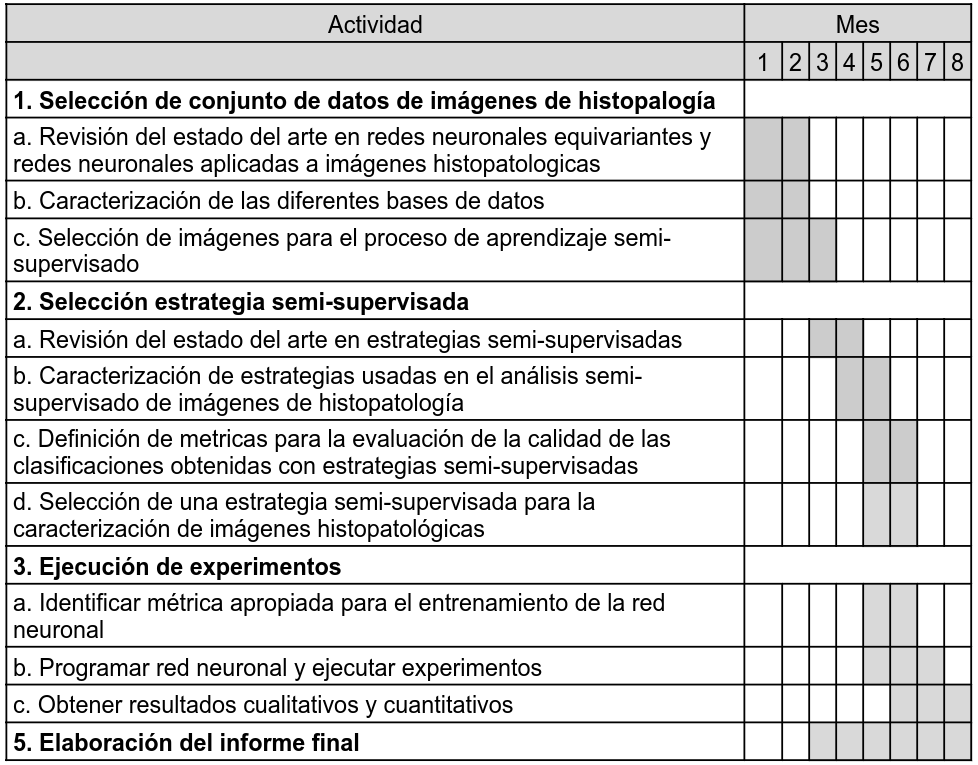
\includegraphics[width=1\textwidth]{Cronograma_max.png}
\end{center}


%% PRESUPUESTO %%%%%%%%%%%%%%%%%%%%%%%%%%%%%%%%%%%%%%%%%%%%%%%%%%%%%%%%%%%%%
\newpage
\chapter{Presupuesto}

% \usepackage{colortbl}
% \usepackage{hhline}
% \usepackage{rotating}


\centering
\begin{tabular}{|c|c|c|c|c|c|}
\hline
\rowcolor[rgb]{0.863,0.863,0.863}  \textbf{Concepto}  & \textbf{Descripción}  & \begin{tabular}[c]{@{}>{\cellcolor[rgb]{0.863,0.863,0.863}}c@{}}\textbf{Fuente de }\end{tabular} & \begin{tabular}[c]{@{}>{\cellcolor[rgb]{0.863,0.863,0.863}}c@{}}\textbf{Valor de}\\\textbf{ referencia*} \end{tabular} & \textbf{Cantidad}  & \begin{tabular}[c]{@{}>{\cellcolor[rgb]{0.863,0.863,0.863}}c@{}}\textbf{Precio}\\\textbf{ estimado} \end{tabular} \\
\hline
Director & Profesor de planta & Especie & \begin{tabular}[c]{@{}c@{}}\$305.000\\ por hora \end{tabular} & \begin{tabular}[c]{@{}c@{}}12/h al mes\\ por 8 meses \end{tabular} & \$29.280.000 \\
\hline
Autor & \begin{tabular}[c]{@{}c@{}}Estudiante de\\ pregrado \end{tabular} & \begin{tabular}[c]{@{}c@{}}Efectivo\\ (Financiación\\ estudiantil) \end{tabular} & \begin{tabular}[c]{@{}c@{}}1 SMMLV\\ por mes \end{tabular} & 12 meses & \$13.920.000 \\
\hline
\begin{tabular}[c]{@{}c@{}}Base de Datos\\ Bibliográfica \end{tabular} & \begin{tabular}[c]{@{}c@{}}Contrapartida\\ UIS \end{tabular} & Especie & \begin{tabular}[c]{@{}c@{}}\$0.000.000\\ al año \end{tabular} & 1 año & \$20.000.000 \\
\hline
Insumos & Papelería & A cargo del autor & - & - & \$200.000 \\
\hline
Transporte & \begin{tabular}[c]{@{}c@{}}Traslados a la\\ universidad \end{tabular} & A cargo del autor & - & - & \$1.000.000 \\
\hline
\multicolumn{1}{l}{} & \multicolumn{1}{l}{} & \multicolumn{1}{l}{} & \multicolumn{1}{l|}{} & {\cellcolor[rgb]{0.863,0.863,0.863}}\textbf{TOTAL}  & \multicolumn{1}{l|}{\$64.400.000} \\
\end{tabular}
\renewcommand*{\thefootnote}{\fnsymbol{footnote}}
\footnotetext[1]{Valores tomados de los rubros presupuestales estipulados por la Vicerrectoría de Investigación y Extensión de la Universidad Industrial de Santander.}








%% REFERENCIAS %%%%%%%%%%%%%%%%%%%%%%%%%%%%%%%%%%%%%%%%%%%%%%%%%%%%%%%%%%%%%
\newpage
%\chapter{Bibliografía}
\bibliographystyle{IEEEtr}
\bibliography{referencias2}

\end{document}
